\documentclass[titlepage]{article}

\title{NATuG User Manual}
\author{Wolf S. Mermelstein and William B. Sherman}

\usepackage{graphicx}
\usepackage{hyperref}
\usepackage{subcaption}
\usepackage{wrapfig}
\usepackage[margin=1in]{geometry}
\graphicspath{{resources/images}} % all graphics will come from the resources/images folder

\begin{document}
	\maketitle
	\tableofcontents 
	\newpage
	
	\section{Getting NATuG Running}
	
	The quick start guide is the fastest way to get NATuG running on any Mac, Windows, or Linux machine. These steps are by no means comprehensive, and are merely a guide to get the program running.
	
	\begin{figure}[h] 
		\centering
		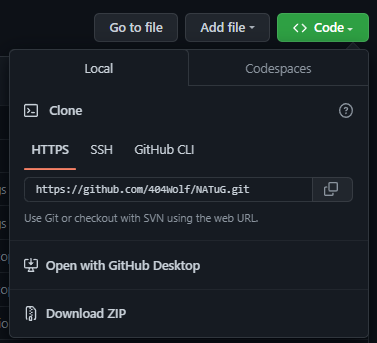
\includegraphics[width=2in]{github-download-menu.png}
		\caption{Github code download menu}
		\label{fig:github-download-menu}
	\end{figure}
	
	\begin{enumerate} \label{sect:getting-natug-running}
		\item Visit \href{Python's download page}{www.python.org/downloads}, and then install the most recent version of Python for your operating system. NATuG has been confirmed to work on versions up to Python 3.11.1
		\item Go to the \href{NATuG’s Github page}{github.com/404Wolf/NATuG}, click the green "code" button, and then click "download ZIP." See Figure~\ref{fig:github-download-menu}.
		\item Open your computer’s terminal/console/command prompt. Enter the following commands, in the following order. 
		
		\begin{enumerate}
			\item “cd $<$filepath$>$” to enter the directory of the project. \label{enum:enter-directory}
			\item “python~-m~venv~venv” to create a virtual environment for the needed libraries to go into.
			\item “venv/Scripts/activate” if you are on windows, or “source~myenv/bin/activate” if you are on Mac/Linux, to enter into the virtual environment. You will know that you have successfully entered the virtual environment if the current line in terminal begins with “(venv).” \label{enum:activate-venv}
			\item “python -m pip install -r requirements.txt” to automatically install all the needed libraries. They may take a while to download.
			\item “python -m launcher” to run the program. The first launch may take a bit while the code compiles. \label{enum:run-program}
		\end{enumerate}
	
		\item You should now be in NATuG! When running the program in the future, simply CD into the folder (step~\ref{enum:enter-directory}), enter the virtual environment (step~\ref{enum:activate-venv}), and run the program (step~\ref{enum:run-program}).
	\end{enumerate}

	\section{Quickstart}
	
	Constructing a DNA nanotube is a complex, multi-stage process, but NATuG streamlines the steps. Below is a quick list of things to do that should help you gain a basic level familiarity with NATuG. 
	
	\textbf{Disclaimer:} The below tasks are by no means comprehensive, and are meant to serve as a simple introduction to the program.
	
	\subsection{Running NATuG}
	First, go to Section~\ref{sect:getting-natug-running} and follow the instructions to get NATuG running.
	
	\subsection{Nucleic Acid Selection}
	
	On the right side of the screen, in the config panel, you will find the Nucleic Acid settings tab. This is the area in which settings for the geometry of your DNA. While most of the time you will use NATuG's default provides for DNA settings, now is a good time to experiment with the different inputs. As you change the different settings, also look at the bottom of the NATuG's window---the Status Bar--when hovering over them. It should display a brief explanation of what the different settings actually are. Observe the Side View Plot and Top View Plot change as the settings update.
	
	\begin{figure}[h]
		\caption{Experimenting with Nucleic Acid settings}
		\centering
		\begin{subfigure}{.5\textwidth}
			\centering
			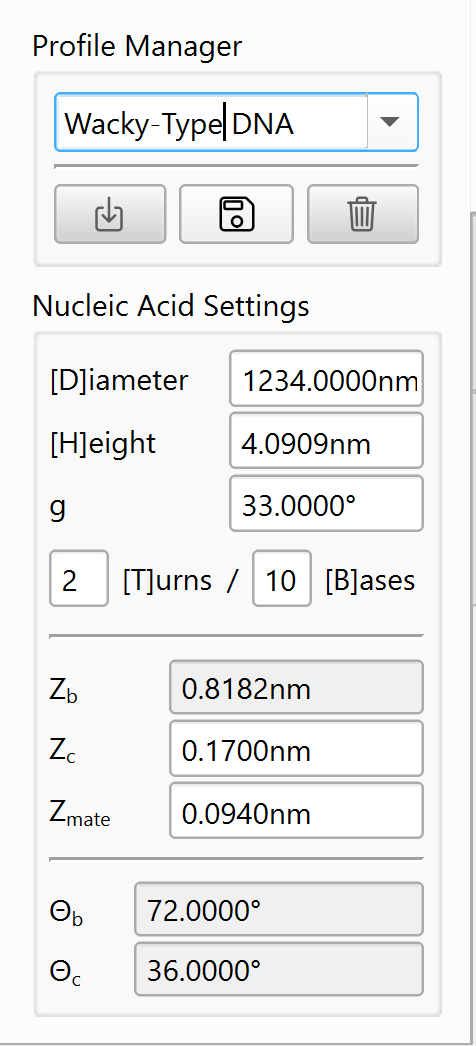
\includegraphics[height=1.7in]{nucleic-acid-tinkering.png}
			\caption{Tinkering With Nucleic Acid Settings}
		\end{subfigure}%
		~
		\begin{subfigure}{.5\textwidth}
			\centering
			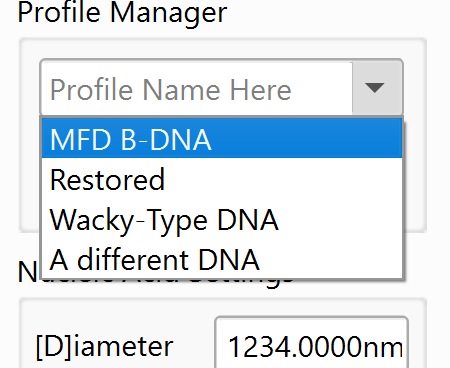
\includegraphics[width=1.7in]{nucleic-acid-tinkering-2.png}
			\caption{Loading different Nucleic Acid profiles}
		\end{subfigure}
	\end{figure}
		
	\subsection{Domain Adjustment}
	
	In the config panel on the right side of the screen, switch to the Domains tab. The panel will pop out because of the required width of the tab. The panel may appear intimidating at first, but you should start by using the small arrow buttons next to the "m" of each domain. As you do so, watch the Top View Plot update in real time. By increasing/decreasing the "m" values, the interior angles of domains will change, which will in turn change the shape of the tube. You can type numbers directly into the boxes, but without correcting for changes with other domains' angles, the tube will open up. Notice how when the tube is closed the M/R box in the symmetry section of the tab lights up green.
	
	In the settings area above the domains table, click the load button (the button that has an arrow pointing downwards into a box). Choose a different set of domains, for instance, "nested.csv." As you play around with this section of NATuG, you can use the save button to save your own designs/your adjustments to the default designs.
		
	\begin{figure}[h]
		\caption{Changing up domain settings}
		\centering
		\begin{subfigure}{.5\textwidth}
			\centering
			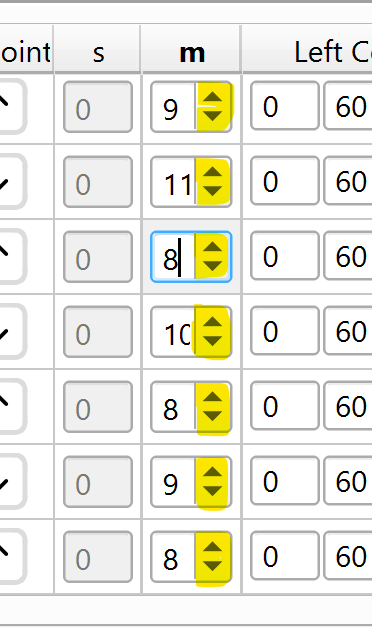
\includegraphics[height=2in]{changing-theta-ms.png}
			\caption{Changing domains' $\theta_{m}$s}
		\end{subfigure}%
		~
		\begin{subfigure}{.5\textwidth}
			\centering
			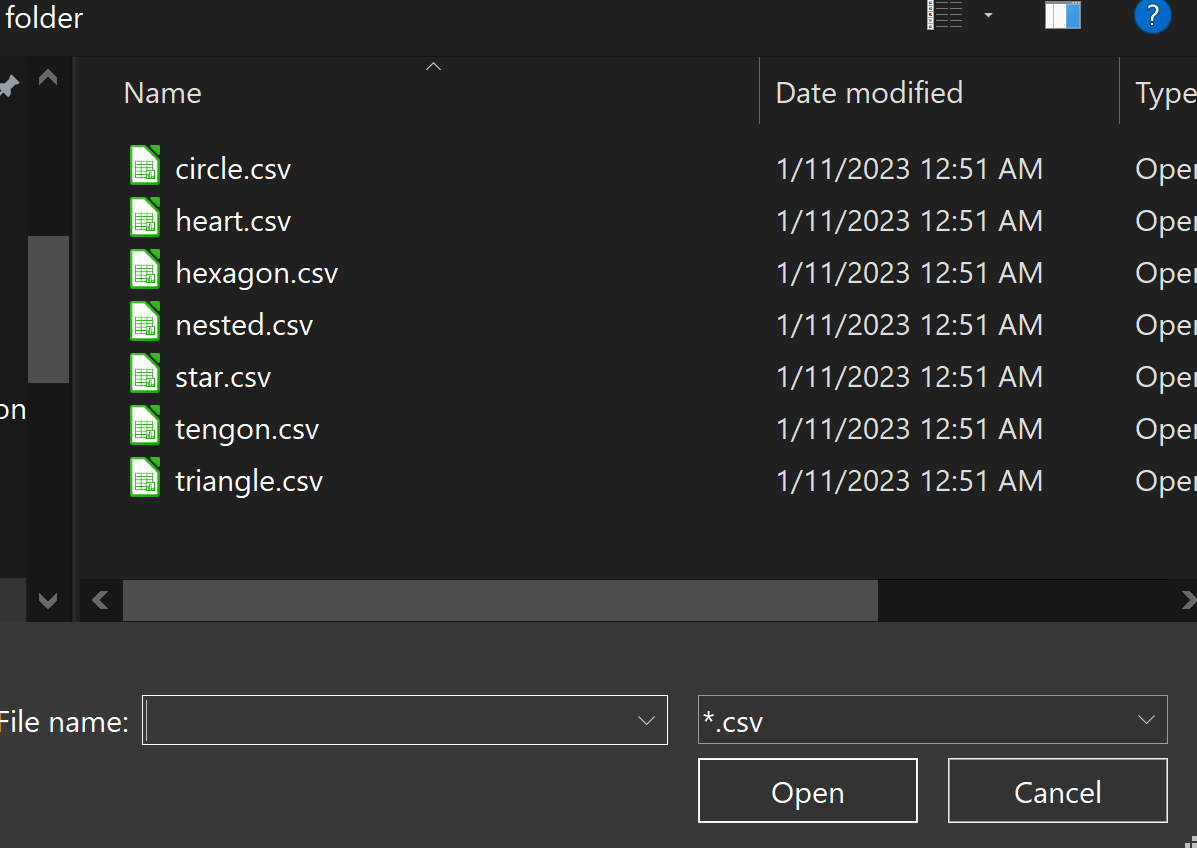
\includegraphics[width=2in]{loading-domains.png}
			\caption{Loading in different domain presets}
		\end{subfigure}
	\end{figure}
		
	\subsection{Junction Creation}
	\begin{figure}[h]
		\centering
		\caption{Creating cross-strand junctions}
		\label{fig:creating-junctions}
		
		\begin{subfigure}{.3\textwidth}
			\centering
			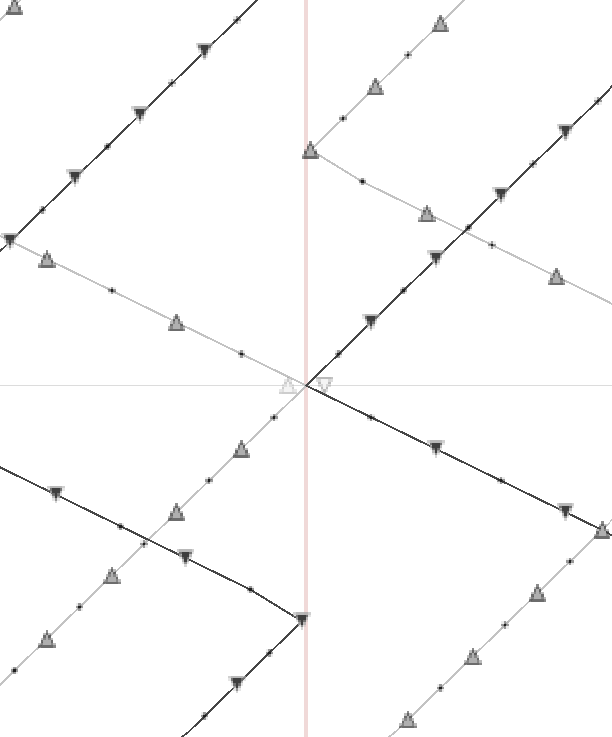
\includegraphics[height=1.7in]{creating-junctions-1.png}
			\caption{Domains with overlapping NEMids}
		\end{subfigure}%
		~
		\begin{subfigure}{.3\textwidth}
			\centering
			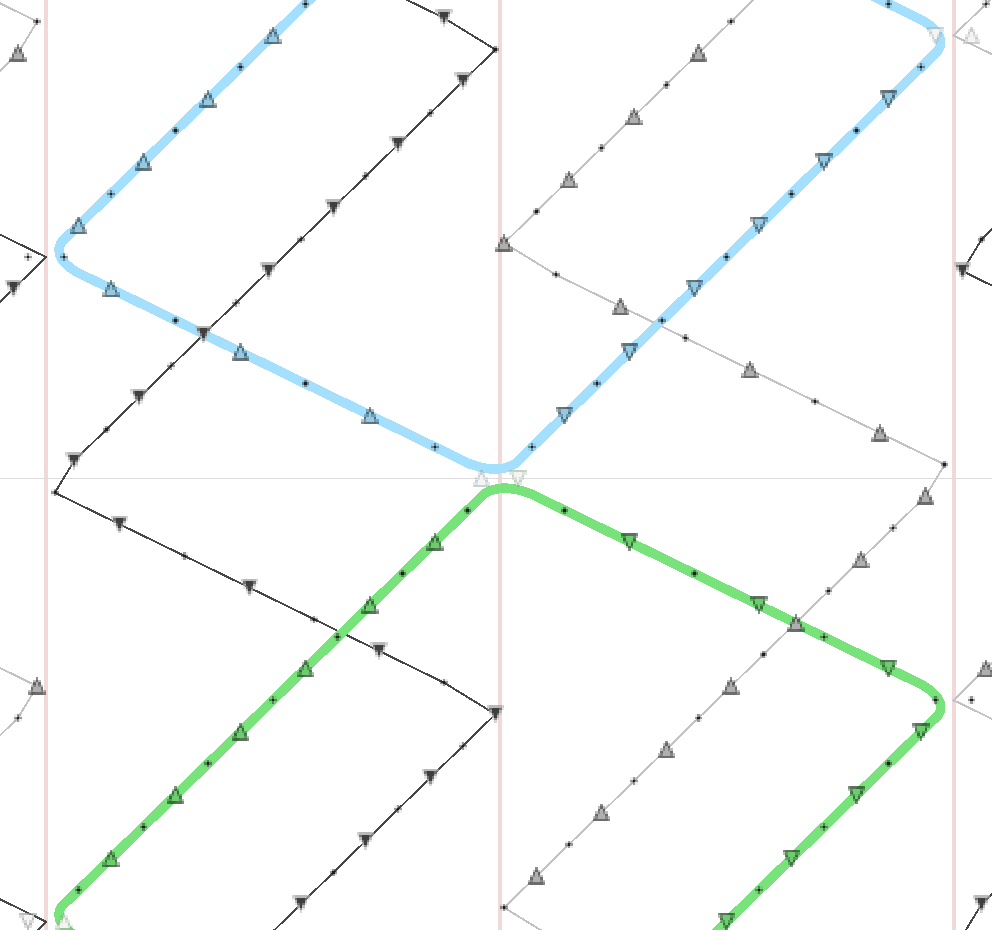
\includegraphics[height=1.7in]{creating-junctions-2.png}
			\caption{Domains with inter-domain strands}
		\end{subfigure}%
		~
		\begin{subfigure}{.3\textwidth}
			\centering
			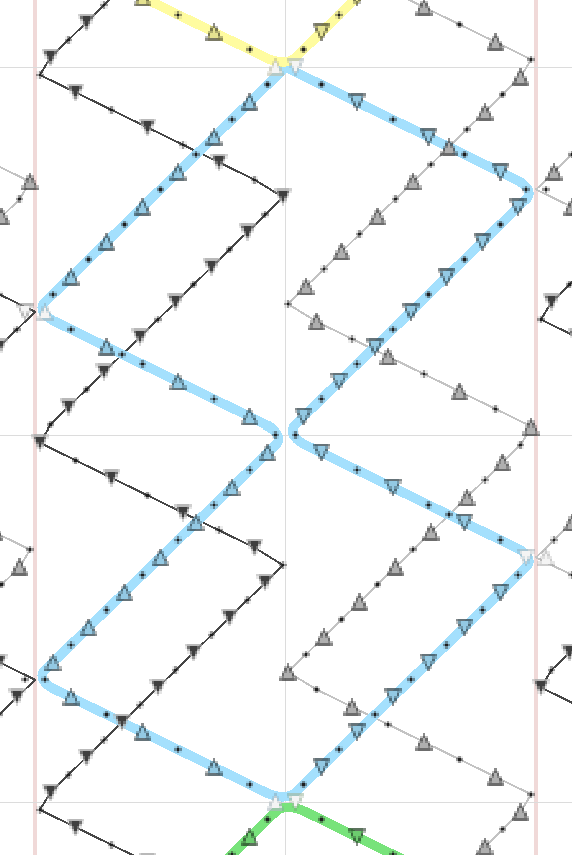
\includegraphics[height=1.7in]{creating-junctions-3.png}
			\caption{Domains with a closed-loop strand and inter-domain strands}
		\end{subfigure}
	\end{figure}
	
	In the Side View Plot---the main area of NATuG---locate two white triangles (which represent the middle of two nucleosides, and are called "NEMids") that are overlapping, and click on them. This will transform two helices of two different domains into two helices that traverse both of the domains. Continuing clicking on overlapping white triangles to weave together strands. See Figure~\ref{fig:creating-junctions} for a visual example.
	
	\subsection{Nicks, Linkages, and Sequences}
	Here, you can begin to experiment with more advanced features of NATuG. You just experimented with creating junctions, but the Side View Plot mode that creates junctions ("juncter" mode) is one of many modes. To try out other modes, go to the top of the window, where you see a list of different buttons ("Informer," "Juncter," "Nicker," etc.), and click on different modes. Then left click on points within the main plot. Below is a list of (very) simplified descriptions of the different modes and how to get started using them.
	
	\begin{figure}[h]
		\caption{Advanced NATuG features}
		\centering
		\begin{subfigure}{.3\textwidth}
			\centering
			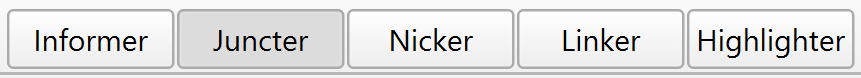
\includegraphics[width=1.4in]{juncter-activated.png}
			\caption{There are other modes!}
		\end{subfigure}%
		~
		\begin{subfigure}{.3\textwidth}
			\centering
			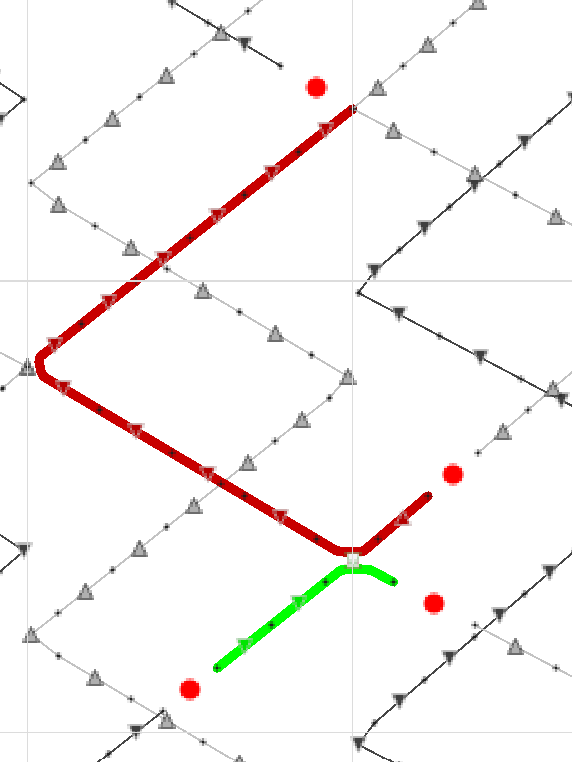
\includegraphics[height=1in]{nick-examples.png}
			\caption{Examples of nicks}
		\end{subfigure}%
		~
		\begin{subfigure}{.3\textwidth}
			\centering
			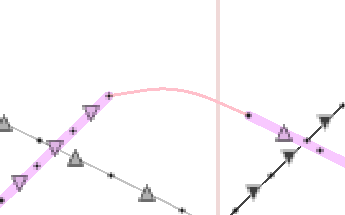
\includegraphics[width=1.5in]{linkage-example.png}
			\caption{Example of linkages}
		\end{subfigure}
	\end{figure}
	
	\begin{enumerate}
		\item \textbf{Informer Mode:} Obtain information about points. To use, click on any point.
		\item \textbf{Juncter Mode:} Redirect strands across helical domains. To use, click on any two overlapping white triangles.
		\item \textbf{Nicker Mode:} Split strands in half. To use, click on any point.
		\item \textbf{Linker Mode:} Link the ends of two strands together to make one bigger strand. To use, click on one point that is at the end of a strand, and then another point that is at the end of a strand. Make sure that the arrows do not point towards each other.
		\item \textbf{Highlighter Mode:} Highlight points. To use, click on any point.
	\end{enumerate}

	\section{Overall Layout}
	
	NATuG’s interface consists of a main hub area, surrounded by two panels. There is a status bar at the bottom of NATuG, which provides helpful descriptions of what various buttons and input boxes do as you hover over them, and a file bar at the top of NATuG, which provides access to various cross-program functions.
	
	\begin{figure}[h]
		\centering
		\caption{The overall layout of NATuG}
		\label{program-layout}
		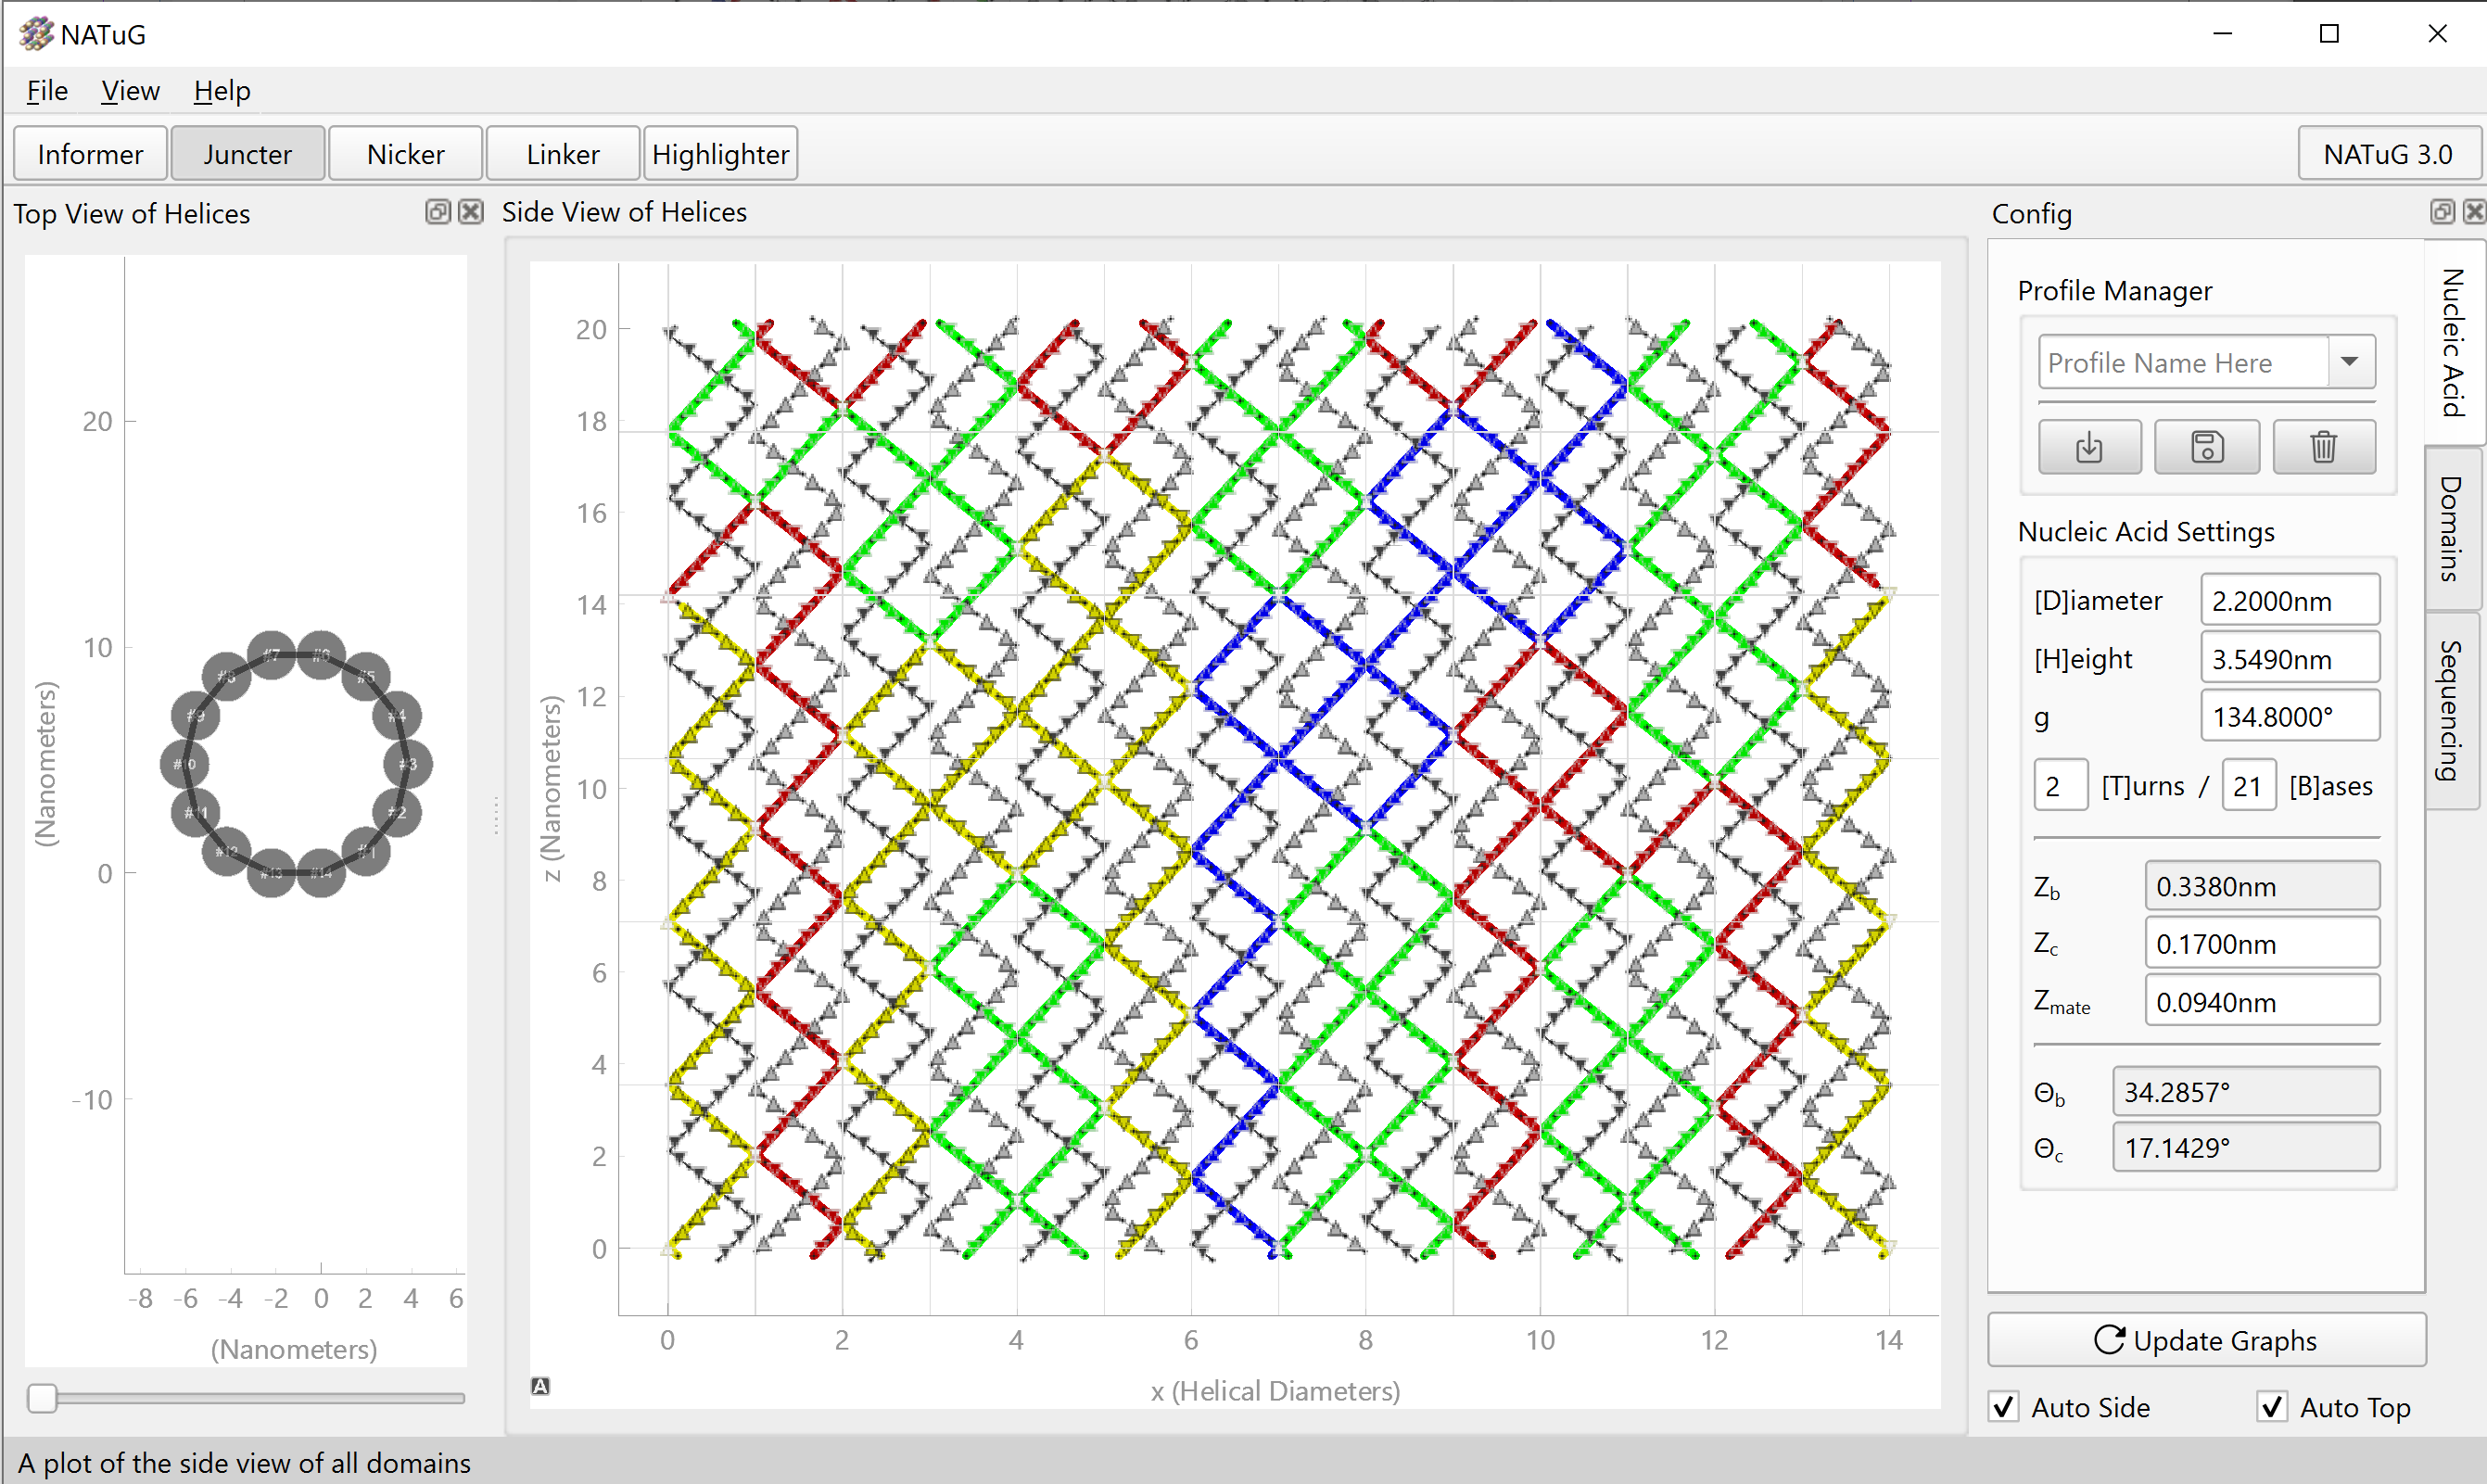
\includegraphics[width=5in]{program-layout.png}
	\end{figure}

	\subsection{Panels} \label{sect:panels}
	NATuG has two panels: the Top View Panel and the Config Panel. Though the contents of panels differ, they do share various important properties:
	
	\begin{enumerate}
		\item Panels are all undockable. By clicking twice on the top area of a panel, or by dragging the panel away from the main window, or by clicking the  button, one can make a panel become its own window. To redock, click on the top of the panel twice, or drag the panel back into the main window. 
		\item Panels are hideable. By clicking the "x" button in the top corner of a panel, or by going to the file menu, "view," and then the name of the panel you are trying to hide, you can hide the panel. To unhide a panel, go to the file menu, "view," and then the name of the panel you are trying to unhide. 
	\end{enumerate}

	\subsection{Hub}
	NATuG’s main area, the “hub,” is another name for the area of the program where the Side View plot is located. Located directly above the Hub is the toolbar, where you can select the current mode of NATuG. Each mode changes what a left click does in the Side View plot.
	
	\section{Config Panel} \label{section:config-panel}
	The Config Panel contains most of the user input areas of NATuG. Within the panel are three primary modes: “Nucleic Acid,” “Domains,” and “Sequencing,” outlined in greater depth on the following pages. 
	
	To navigate between panels of the config panel, simply click on one of the tabs. Below are brief descriptions of the various tabs; however, each tab has a dedicated page as well.
	
	\textbf{Warning:} changing settings within the config panel will reset all current junctions, nicks, links, and highlights. Attempting to change settings when there exist any junctions, links, or highlights will result in a popup dialog that offers to save the current state of the Side View Plot and then refresh the plot, refresh the plot without saving, or cancel the attempted refresh.
	
	\begin{figure}[h]
		\centering
		\includegraphics[width=3in]{"nucleic-acid-tab-activated.png"}
		\label{fig:nucleic-acid-tab-activated}
	\end{figure}

	The Nucleic Acid Tab is where one can customize the geometrical settings of the nucleic acid that they are creating a nanotube for. This defaults to B type DNA, and generally does not need to be changed. 

	\begin{figure}[h]
		\centering
		\includegraphics[width=3in]{"domains-tab-activated.png"}
		\label{fig:domains-tab-activated}
	\end{figure}

	The Domains Tab is where settings for the interior angles, strand switches, and the number of NEMids to generate are inputted. This section allows the user to actually define the shape of the nanotube.

	\begin{figure}[h]
		\centering
		\includegraphics[width=3in]{"sequencing-tab-activated.png"}
		\label{fig:sequencing-activated}
	\end{figure}

	The Sequencing Tab is where the user can apply bulk sequence actions to all the strands, and export sequences to a spreadsheet for synthesis. This is generally one of the later steps in the nanotube design process.
	
	\subsection{Graph Updating}
	
	By default, as changes are made within the various tabs of the Config Panel the Side View Plot and Top View Plot automatically update. To disable automatic updating for either plot, click either of the “Auto Side” or “Auto Top” buttons on the bottom of the Config panel. When automatic updating is disabled, the “Update Graphs” button must be clicked to refresh the plots. Manual updating can be useful for larger structures that take a long time to load.
	
	The current tab of the Config Panel determines what is currently plotted in the Side View Plot. When the current tab is either “Nucleic Acid” or “Domains” NEMids are plotted, and the mode of the Side View Plot is unrestricted. However, when “Sequencing” is active, nucleosides are plotted. When this is the case, only the “highlighter” and “informer” modes are enabled within the Side View Plot’s toolbar.
	
	\subsection{Nucleic Acid Tab} \label{sect:nucleic-acid-tab}
	
	The Nucleic Acid Tab is the area in which all geometrical settings for the nucleic acid being used can be entered. All of NATuG’s computations utilize these constants, so only make changes if you know what you are doing. This tab contains a profile manager for easily loading in sets of settings, and has various fields that warrant extended descriptions. When using NATuG, recall that hovering over fields will show additional information in the Status Bar at the bottom of the window---this feature is particularly useful for the Nucleic Acid Tab because hovering over setting fields shows descriptions in the status bar of what they represent.
	
	\subsubsection{Profile Manager}
	
	The profile manager lets you easily save and load various sets of nucleic acid settings. Using NATuG’s profile defaults will ensure that all the settings are correct, and you can also create your own profiles for future use.
	
	By default, NATuG includes common profiles, such as one for B type DNA. Profiles are saved internally, and can easily be loaded/retrieved, and .json files containing the profile data can be found within the saves/nucleic\_acid folder. These files are loaded when NATuG is booted, and can be modified directly. Additionally, when NATuG is closed, the last used settings are saved, and are automatically retrieved upon the next launch.
	
	To use the profile manager, enter the name of the profile you would like to save/load/delete into the “Profile Name Here” box, and click the respective button. For extended descriptions of what each button does, see below. When a profile manager box is disabled/gray, consult the status bar for information as to why. For irreversible actions warnings will be shown before the action is run. Below is a list of more extended descriptions of the various profile manager actions.
	
	\begin{figure}
		\caption{Various Profile Actions}
		
		\centering
		\begin{subfigure}{.3\textwidth}
			\centering
			\caption{The load profile button}
			
\includegraphics[width=1in]{load-profile-button.png}
			\label{fig:load-profile-button}
		\end{subfigure}%
		~
		\begin{subfigure}{.3\textwidth}
			\centering
			\caption{The save profile button}
			
\includegraphics[width=1in]{save-profile-button.png}
			\label{fig:save-profile-button}
		\end{subfigure}%
		~
		\begin{subfigure}{.3\textwidth}
			\centering
			\caption{The delete profile button}
			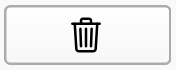
\includegraphics[width=1in]{delete-profile-button.png}
			\label{fig:delete-profile-button}
		\end{subfigure}
	\end{figure}
	
	\paragraph{Load Profile}
	Load the profile with the currently chosen profile name. This requires a profile to already exist with the name chosen, and for the current settings to not be the  the settings of that profile. (Icon~\ref{fig:load-profile-button})
	
	\paragraph{Save Profile}
	Save the profile with the currently chosen profile name, or, if there is already a profile with that name, overwrite the existing profile. The profile will be saved to a .json file within saves/nucleic\_acid after the program is closed. (Icon~\ref{fig:save-profile-button})
	
	\paragraph{Delete Profile}
	Delete the profile with the currently chosen profile name. This action is irreversible. Default profiles cannot be deleted. (Icon~\ref{fig:delete-profile-button})

	\subsubsection{Setting Descriptions}
	Below lies a list of all of the various Nucleic Acid settings that can be adjusted. Certain settings (the ones that are have an "(a)" in the table) are automatically determined based on other settings and cannot be user set. \linebreak
	
	\begin{center}
	\begin{tabular}{|p{.5in}|p{1in}|p{.7in}|p{1.5in}|}
		\label{tab:setting-descriptions}
		Input & Name & Data Type & Description \\
		\hline
		$D$ & Diameter & number & The diameter of a given domain in nanometers \\ \hline
		$H$ & Height & number & The height of one turn of the helical axes \\ \hline
		$g$ & Nucleoside-Mate Angle & number between 0 and 360 & The angle about the helical axis between a nucleoside and its Watson-Crick mate \\ \hline
		$T/B$ & Helical Turns per Bases & integers & There are T turns every B bases \\ \hline
		$Z_b$ (a) & Base Height & number & The height between two NEMids on a given helix \\ \hline
		$Z_c$ & Characteristic Angle & number & The height a helix climbs as it rotates through the characteristic angle \\ \hline
		$Z_{mate}$ & Nucleoside-Mate Height & number & Vertical distance between a NEMid and its mate on the other helix. \\ \hline
		$\theta_{c}$ (a) & Characteristic Angle & number between 0 and 360 & The smallest angle about the helical axis possible between two NEMids on the same helix. \\ \hline
		$\theta_{b}$ (a) & Interbase Angle & number between 0 and 360 & The angle that about the helical axis between two NEMids \\
	\end{tabular}
	\end{center}
	
	\subsection{Domains}
	
	\begin{figure}[h]
		\centering
		\caption{Domains Config Table}
		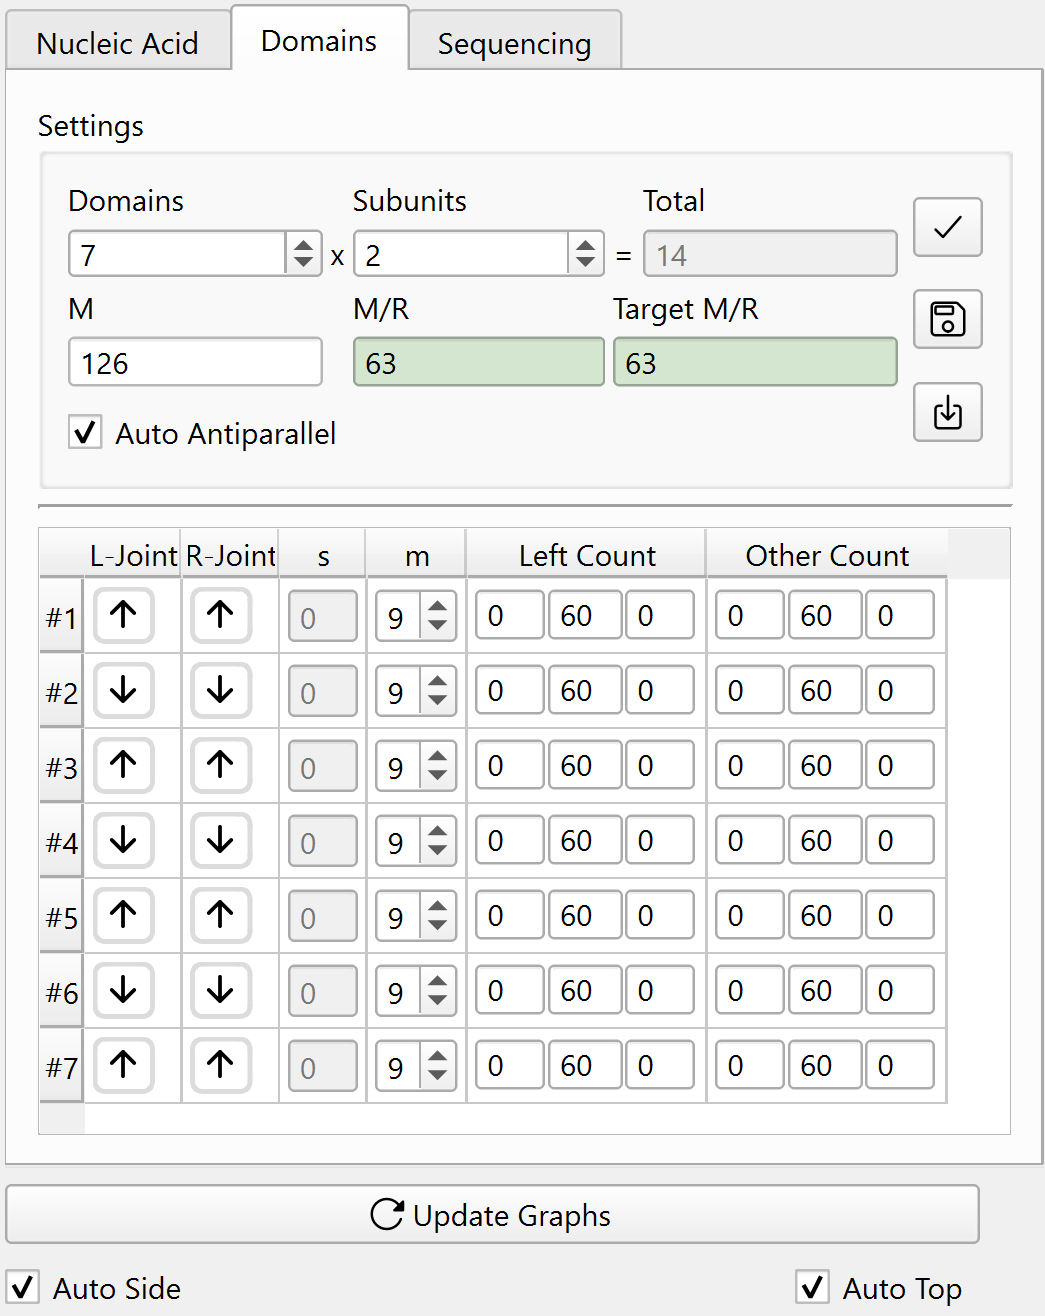
\includegraphics[height=2.5in]{domain-config-table.png}
		\label{fig:domain-config-table}
	\end{figure}

	The Domains Tab is the area in which all the settings for each helical domain can be set. The angles between each domain are what determine what the ultimate shape of the nanostructure will be. NATuG provides support for symmetrical designs, saving and loading designs, and provides tools for designing closed structures.
	
	\begin{itemize}
		\item "M" represents the sum of all of the little "m"s for each domain in the Table Area.
		\item "R" represents the number of subunits, and a green "M/R" box indicates that the tube is closed.
		\item To create sticky ends, adjust the left/rightmost boxes of the “Left/Other Count” columns. For more information, see "Settings Descriptions"
	\end{itemize}
	
	\subsection{Sequencing}
	
	\begin{figure}
		\centering
		\caption{Sequencing Tab}
		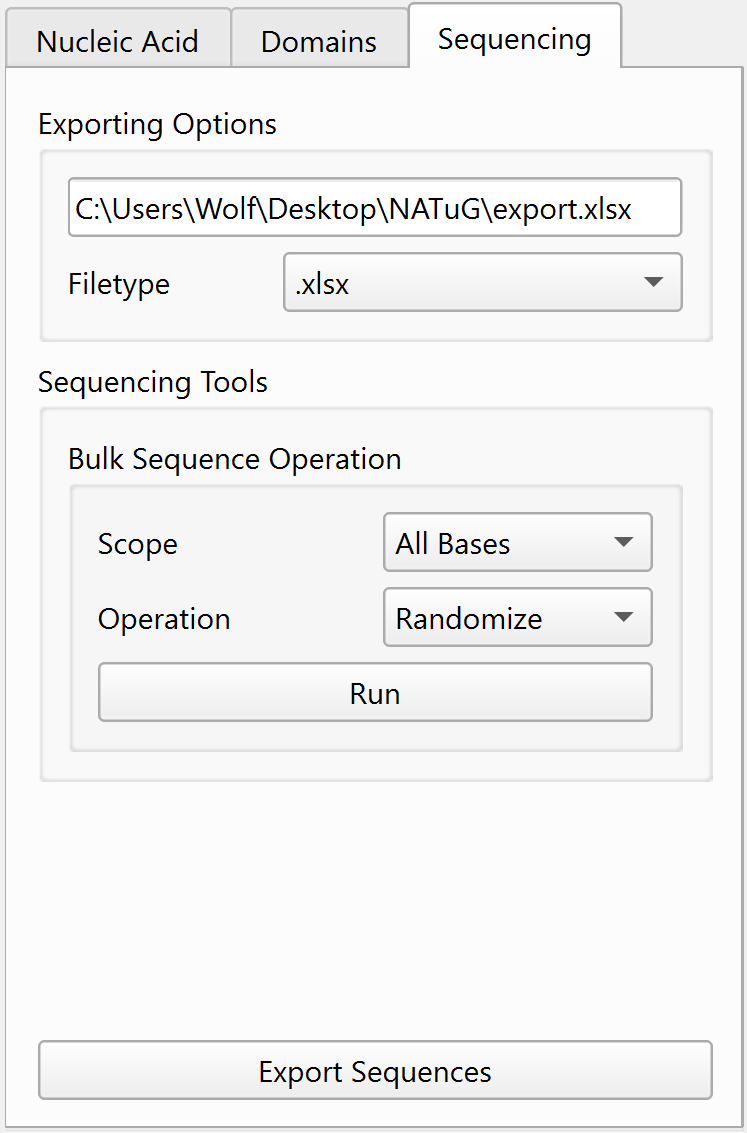
\includegraphics[height=2.4in]{sequencing-tab.png}
		\label{fig:sequencing-tab}
	\end{figure}
	
	This tab allows for bulk sequence operations, and for exporting sequences to a spreadsheet for synthesis. Because sequencing is such a critical part of NATuG, it has a section that goes into greater depth about how it works. It is also important to note that this is not the only place where sequences can be set. For more information about sequencing, consult section~\ref{sect:sequence-selector}.
	
	\subsubsection{Bulk Sequence Operations}
	Bulk sequence operations let you set the sequence of many nucleosides at once. In order to run a bulk sequence operation, select a "Scope," then an "Operation," and then click "Run."
	
	\paragraph{Scopes}
	The scope is which nucleosides the operation should run on.
	
	\begin{itemize}
		\item \textbf{All bases:} All the nucleosides of all the strands.
		\item \textbf{Unset bases:} All the nucleosides of all the strands that do not currently have a base set.
	\end{itemize}

	\paragraph{Operations}
	The operation is what to do to the nucleosides within the scope.
	
	\begin{itemize}
		\item \textbf{Randomize:} Select random bases.
		\item \textbf{Clear:} Unset the bases.
	\end{itemize}
	
	\section{Side View Plot}
	The Side View Plot is the heart of NATuG. It allows you to directly interact with strands that have been created as a result of user inputs set elsewhere. The plot can be broken into a few distinct parts that function together to allow for a high degree of interactivity. 
	
	\begin{figure}[h]
		\centering
		\caption{The Side View Plot \& toolbar}
		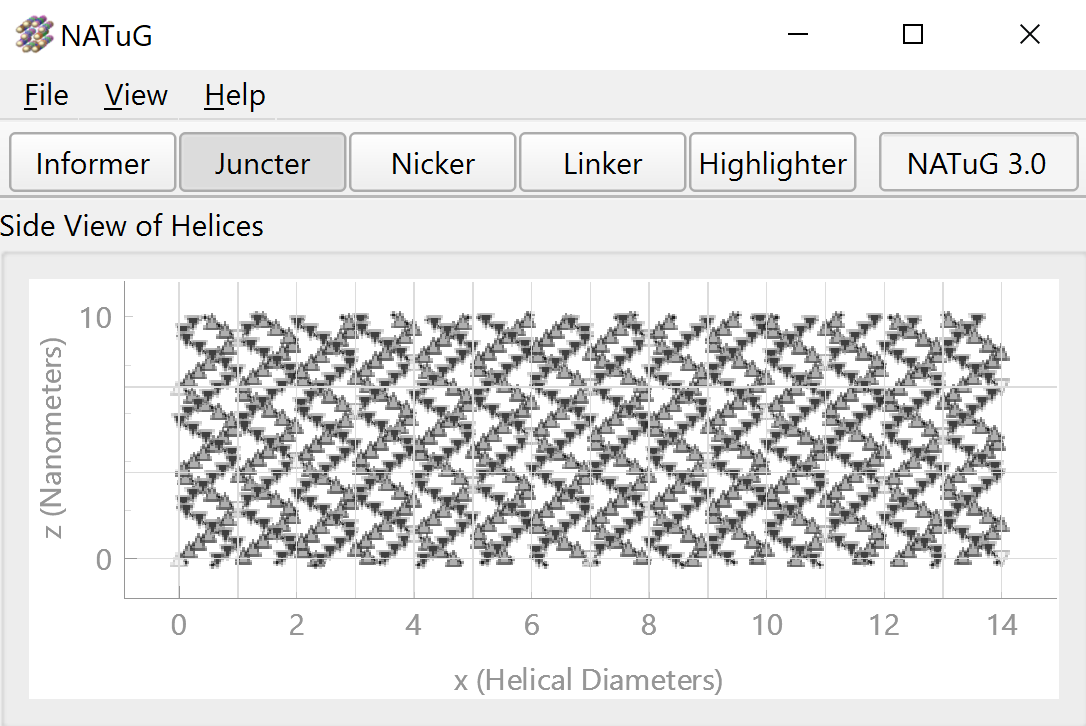
\includegraphics[width=4in]{short-side-view-overview.png}
		\label{fig:short-side-view-overview}
	\end{figure}

	\subsection{Graphics}
	Before diving into how to actually interact with the Side View Plot, it is important to understand what the contents of the plot actually represent. The Side View Plot is not, as its name implies, a direct side view of the double helices. Rather, it is more of an “unrolled” plot, since it is distorted in such a way as to neatly lay out the double helices next to one another.
	
	Importantly, the plot consists of various artifacts, which represent physical nucleosides, or abstract areas between physical nucleosides. Below lies further descriptions of what these artifacts are.
	
	\subsubsection{Points}
	
	\begin{figure}[h]
		\centering
		\caption{Side View Plot Point Graphics}
		\label{fig:side-view-plot-point-graphics}
		
		\begin{subfigure}{.3\linewidth}
			\centering
			
\includegraphics[width=.3in]{up-triangle.png}
			\caption{Triangle Point}
			\label{fig:up-triangle}
		\end{subfigure}%
 		~
		\begin{subfigure}{.3\linewidth}
			\centering
			
\includegraphics[width=.3in]{base-symbol.png}
			\caption{Letter Point}
			\label{fig:base-symbol}
		\end{subfigure}%
		~
		\begin{subfigure}{.3\linewidth}
			\centering
			
\includegraphics[width=.3in]{nondominant-point.png}
			\caption{Circle Point}
			\label{fig:nondominant-point}
		\end{subfigure}
	\end{figure}

	If the Config Panel's (\ref{section:config-panel}) current tab is set to either "Nucleic Acid" or "Domains":
	\begin{itemize}
		\item The triangles represent NEMids. The direction the triangles point (up/down) indicates the direction of the strand. White triangles represent two overlapping NEMids that are clickable, and, when clicked, can form a cross-strand exchange.
		\item The dots represent nucleosides, and cannot be interacted with.
	\end{itemize}

	If the Config Panel's (\ref{section:config-panel}) current tab is set to "Sequencing":
	\begin{itemize}
		\item The triangles represent nucleosides with unset bases. The directions the triangles point (up/down) indicates the direction of the strand.
		\item The letters represent nucleosides that have bases set. The letter indicates what the base of the nucleoside is. 
		\item The dots represent NEMids, and cannot be interacted with.
	\end{itemize}

	\subsubsection{Lines}

	\begin{figure}[h]
		\centering
		\caption{Side View Plot Line Graphics}
		\label{fig:side-view-plot-line-graphics}
		
		\begin{subfigure}{.4\linewidth}
			\centering
			
\includegraphics[width=.3in]{strand-line.png}
			\caption{Strand Line}
			\label{fig:strand-line}
		\end{subfigure}%
		~
		\begin{subfigure}{.3\linewidth}
			\centering
			
\includegraphics[width=.3in]{interdomain-strand-line.png}
			\caption{Interdomain Strand Line}
			\label{fig:interdomain-strand-line}
		\end{subfigure}
	\end{figure}

	The lines connecting dots together are not a literal representation of the location of the phosphate backbone of the DNA, but rather serve as a visual aid to see which strands are which. To this end, by default "interdomain" strands (strands that traverse multiple domains) are automatically styled to be thicker and more colorful to stand out—however, the styles of lines are completely customizable.
	
	Additionally, for interdomain strands, the lines are curved (with \href{https://www.cs.unc.edu/~dm/UNC/COMP258/LECTURES/Chaikins-Algorithm.pdf}{Chaikin's Corner Cutting Algorithm}). This is so that it is clear which strand is which, and because with the thicker lines that interdomain strands posses appear to merge with themselves without rounding of corners. At this time, this setting cannot be disabled.
	
	\subsection{Interaction} \label{sect:plot-interaction}
	NATuG utilizes the pyqtgraph framework for its plots. Below lies a general description of the means of interaction for the plot, but, for a more direct and comprehensive breakdown, visit \href{https://pyqtgraph.readthedocs.io/en/latest/user_guide/mouse_interaction.html}{pyqtgraph’s website} (\href{https://pyqtgraph.readthedocs.io/en/latest/user_guide/mouse_interaction.html}{pyqtgraph.readthedocs.io}).
	
	\subsubsection{Panning}
	To pan from left to right within the side view plot, left click, and then drag your cursor away from the area that you want to pan to. You can think of this as “pulling” the graph towards the cursor. Alternatively, if you have a mouse, you also have the option of clicking the scroll wheel and dragging in the direction that you would like to move the plot in.
	
	\subsubsection{Zooming}
	
	To have the plot automatically zoom in out to showcase all of the items currently plotted, click the small "A" symbol in the bottom left of the plot. This is called the "Auto Range" button. For zooming in on specific areas of the plot, see below.
	
	\begin{itemize}
		\item If you have a mouse:
			\begin{itemize}
				\item To zoom while maintaining the aspect ratio of the plot, use the scroll wheel.
				\item To zoom without regard for the aspect ratio of the plot, right click, and then drag in the direction that you would like to stretch the plot in. The axes will automatically update.
			\end{itemize}
	
		\item If you have a trackpad:
			\begin{itemize}
				\item To zoom while maintaining the aspect ratio of the plot, pinch inwards to outwards to zoom in, and outwards to inwards to zoom out.
				\item To zoom without regard for the aspect ratio of the plot, pinch and right click simultaneously. 
			\end{itemize}
	\end{itemize}

	\subsubsection{Configuration}
	For additional options for the plot, right click. Upon right clicking, a small dialog showing additional plot options will show up. This allows for more advanced configuration of how the plot appears.
	
	\subsection{Modes}
	The currently chosen mode dictates what left clicks on non-dot points in the Side View Plot does. To change the mode, simply click on the mode that you would like to change to. Only one mode can be chosen at a time, and the currently chosen mode is indicated in a slightly darker gray than the others.
	
	\subsubsection{Informer Mode}
	
	\begin{figure}[h]
		\caption{Informer Dialogs}
		\centering
		\begin{subfigure}{.3\textheight}
			\centering
			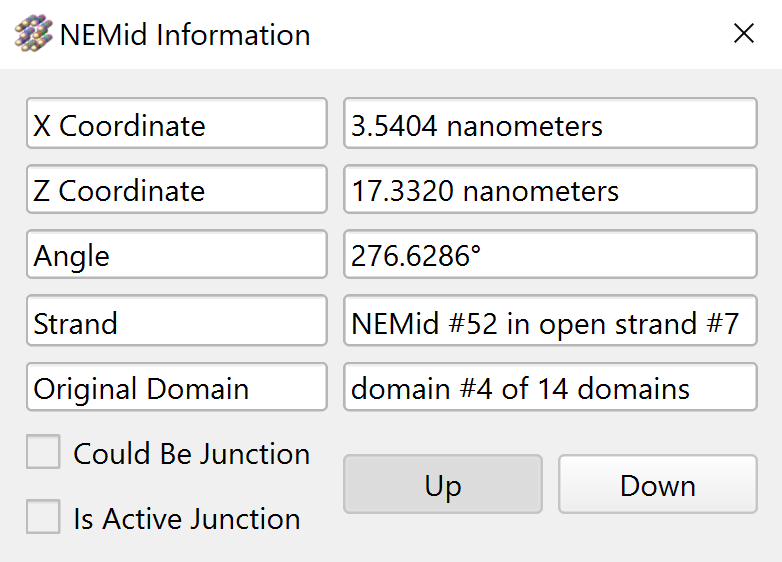
\includegraphics[height=1.3in]{NEMid-informer.png}
			\caption{NEMid Informer Dialog}
			\label{fig:NEMid-informer}
		\end{subfigure}%
		~
		\begin{subfigure}{.3\textheight}
			\centering
			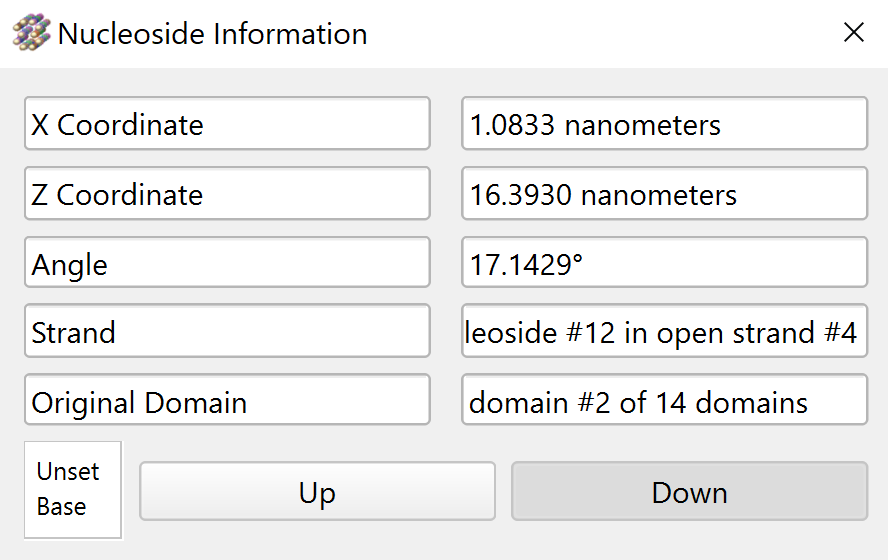
\includegraphics[height=1.3in]{nucleoside-informer.png}
			\caption{Nucleoside Informer Dialog}
			\label{fig:nucleoside-informer}
		\end{subfigure}
	\end{figure}
	
	The "Informer" mode is for obtaining additional information about given points. It provides a dialog that shows various attributes of the point(s) that were clicked on.

	The informer mode is for obtaining additional information about given points. When the informer mode is active, clicking on any point within the main plot will create a dialog that provides additional information about the point. If you click on a NEMid that could be made into a junction, two informers will appear---one for the NEMid that was clicked, and one for the NEMid that that NEMid could potentially be made into a junction with. There are two different types of dialogs: the NEMid Dialog~\ref{fig:NEMid-informer} and the Nucleoside Dialog~\ref{fig:nucleoside-informer}.
	
	\paragraph{Nucleoside Informer} \label{paragraph:nucleoside-informer}
	Descriptions of the various properties that the Nucleoside Informer displays:
	\begin{enumerate}
		\item \textbf{X Coordinate:} The x coordinate of the nucleoside. \label{item:nucleoside-informer-x-coord}
		\item \textbf{Z Coordinate:} The z coordinate of the nucleoside. \label{item:nucleoside-informer-z-coord}
		\item \textbf{Angle:} The angle of the nucleoside. The line of tangency between the previous domain and this domain marks the zero degree mark. This is automatically moduloed by 360. \label{item:nucleoside-informer-angle}
		\item \textbf{Strand:} The index of the nucleoside within its parent strand, and the index of the parent strand within the list of all strands. Indexes begin at \#1. This is the nucleoside index, not the item index, so even though it is true that strands progress nucleoside, NEMid, nucleoside, etc., this index only takes into account nucleosides. \label{item:nucleoside-informer-strand}
		\item \textbf{Original Domain:} The domain that this nucleoside belongs to. \label{item:nucleoside-informer-domain}
		\item \textbf{Base:} The base that this nucleoside is currently set to. If the nucleoside does not have a base set, this box will read "Unset Base."
		\item \textbf{Direction:} The direction of the strand. The darker box is the direction that the strand is going in.  \label{item:nucleoside-informer-direction}
	\end{enumerate}

	\paragraph{NEMid Informer}
	Descriptions of the various properties that the NEMid Informer displays:
	\begin{enumerate}
		\item \textbf{X Coordinate:} Same as Nucleoside Informer \#\ref{item:nucleoside-informer-x-coord}
		\item \textbf{Z Coordinate:} Same as Nucleoside Informer \#\ref{item:nucleoside-informer-z-coord}
		\item \textbf{Angle:} Same as Nucleoside Informer \#\ref{item:nucleoside-informer-angle}
		\item \textbf{Strand:} Same as Nucleoside Informer \#\ref{item:nucleoside-informer-strand}
		\item \textbf{Original Domain:} Same as Nucleoside Informer \#\ref{item:nucleoside-informer-domain}
		\item \textbf{Could Be Junction:} Whether this NEMid could be conjuncted with another NEMid. If this is set to true then clicking on this NEMid in Juncter Mode (\ref{sect:juncter}) will be allowed, otherwise an error will be displayed.
		\item \textbf{Is Active Junction:} Whether this NEMid is currently conjuncted with another NEMid. 
		\item \textbf{Direction:} Same as Nucleoside Informer \#\ref{item:nucleoside-informer-direction}
	\end{enumerate}

	\subsubsection{Juncter Mode} \label{sect:juncter}

	\begin{figure}[h]
		\caption{Junction Sites and Junctable Regions}
		\label{fig:junction-sites}
		
		\begin{subfigure}{.23\linewidth}
			\centering
			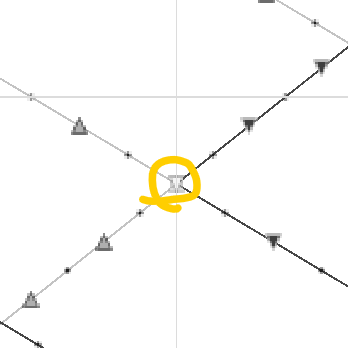
\includegraphics[height=.6in]{junctable-region.png}
			\caption{Two overlaping NEMids}
			\label{fig:junctable-region}
		\end{subfigure}%
		~
		\begin{subfigure}{.234\linewidth}
			\centering
			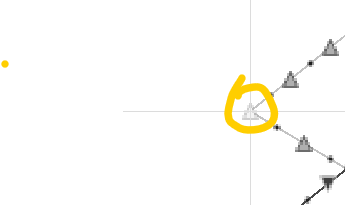
\includegraphics[height=.6in]{cross-screen-junctable.png}
			\caption{Two overlapping cross-screen NEMids}
			\label{fig:cross-screen-junctable}
		\end{subfigure}%
		~
		\begin{subfigure}{.23\linewidth}
			\centering
			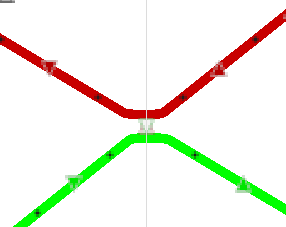
\includegraphics[height=.6in]{active-junction.png}
			\caption{An active junction site}
			\label{fig:active-junction-site}
		\end{subfigure}%
		~
		\begin{subfigure}{.23\linewidth}
			\centering
			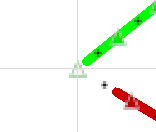
\includegraphics[height=.6in]{cross-screen-junction-site.png}
			\caption{An active cross-screen junction site}
			\label{fig:active-cross-screen-junction}
		\end{subfigure}
	
	\end{figure}

	The "Juncter" mode allows for the creation of cross-strand exchanges. It lets you left click on overlapping NEMids to create junctions. 
	
	There are two ways to create a junction:
	\begin{itemize}
		\item Clicking on two overlapping NEMids (indicated by white triangles that are on top of each other as shown in figure~\ref{fig:junctable-region}). This is the typical type of junction, and is highly versatile---it can split closed loops, form closed loops, allow a strand to go across many domains, and more. See figure~\ref{fig:active-junction-site} for an example of what a junction will look like after a left click.
		\item Clicking on a single NEMid that overlaps a NEMid on the other side of the screen (see figure~\ref{fig:cross-screen-junctable}). This type of junction is called a "cross-screen" junction, and can be seen in figure~\ref{fig:active-cross-screen-junction}. Since the Side View Plot is really an unrolled view of all of the helical domains, the very left for closed structures will sometimes have NEMid overlaps with the very right. 
	\end{itemize}

	\subsubsection{Nicker Mode}
	
	\begin{figure}[h]
		\centering
		\caption{Nick examples}
		\label{fig:nick-examples}
		
		\begin{subfigure}{.4\linewidth}
			\centering
			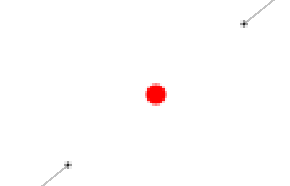
\includegraphics[height=.6in]{nick.png}
			\caption{A nick}
			\label{fig:nick}
		\end{subfigure}%
		~
		\begin{subfigure}{.4\linewidth}
			\centering
			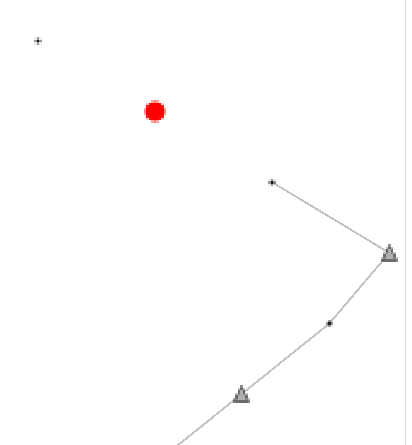
\includegraphics[height=.6in]{end-of-strand-nick.png}
			\caption{A nick at the end of a strand.}
			\label{fig:end-of-strand-nick}
		\end{subfigure}
	\end{figure}

	The "Nicker" mode is how you can create nicks within the strand. Nicks are essentially gaps that split a strand into two different strands.
	
	To create a nick, click on any NEMid, and the NEMid will convert into a red circle. There will then be two strands: one consisting of all of the NEMids and nucleosides that were above the NEMid, and one consisting of all the NEMids and nucleosides below the NEMid. The NEMid itself will be removed.
	
	Notes about nicking:
	\begin{itemize}
		\item When you create a nick the data of the original strand is saved, so, to remove a nick, click on the nick a second time and the original strand will return.
		\item Creating a nick at the end of a strand is unadvised because, as can be seen in figure~\ref{fig:end-of-strand-nick}, you will likely inadvertently create a strand that consists of a single nucleoside.
		\item The nitrogenous bases of all the nucleosides in the two new strands will be preserved.
	\end{itemize}

	\subsubsection{Linker Mode}
	
	\begin{figure}[h]
		\centering
		\caption{The linkage editor}
		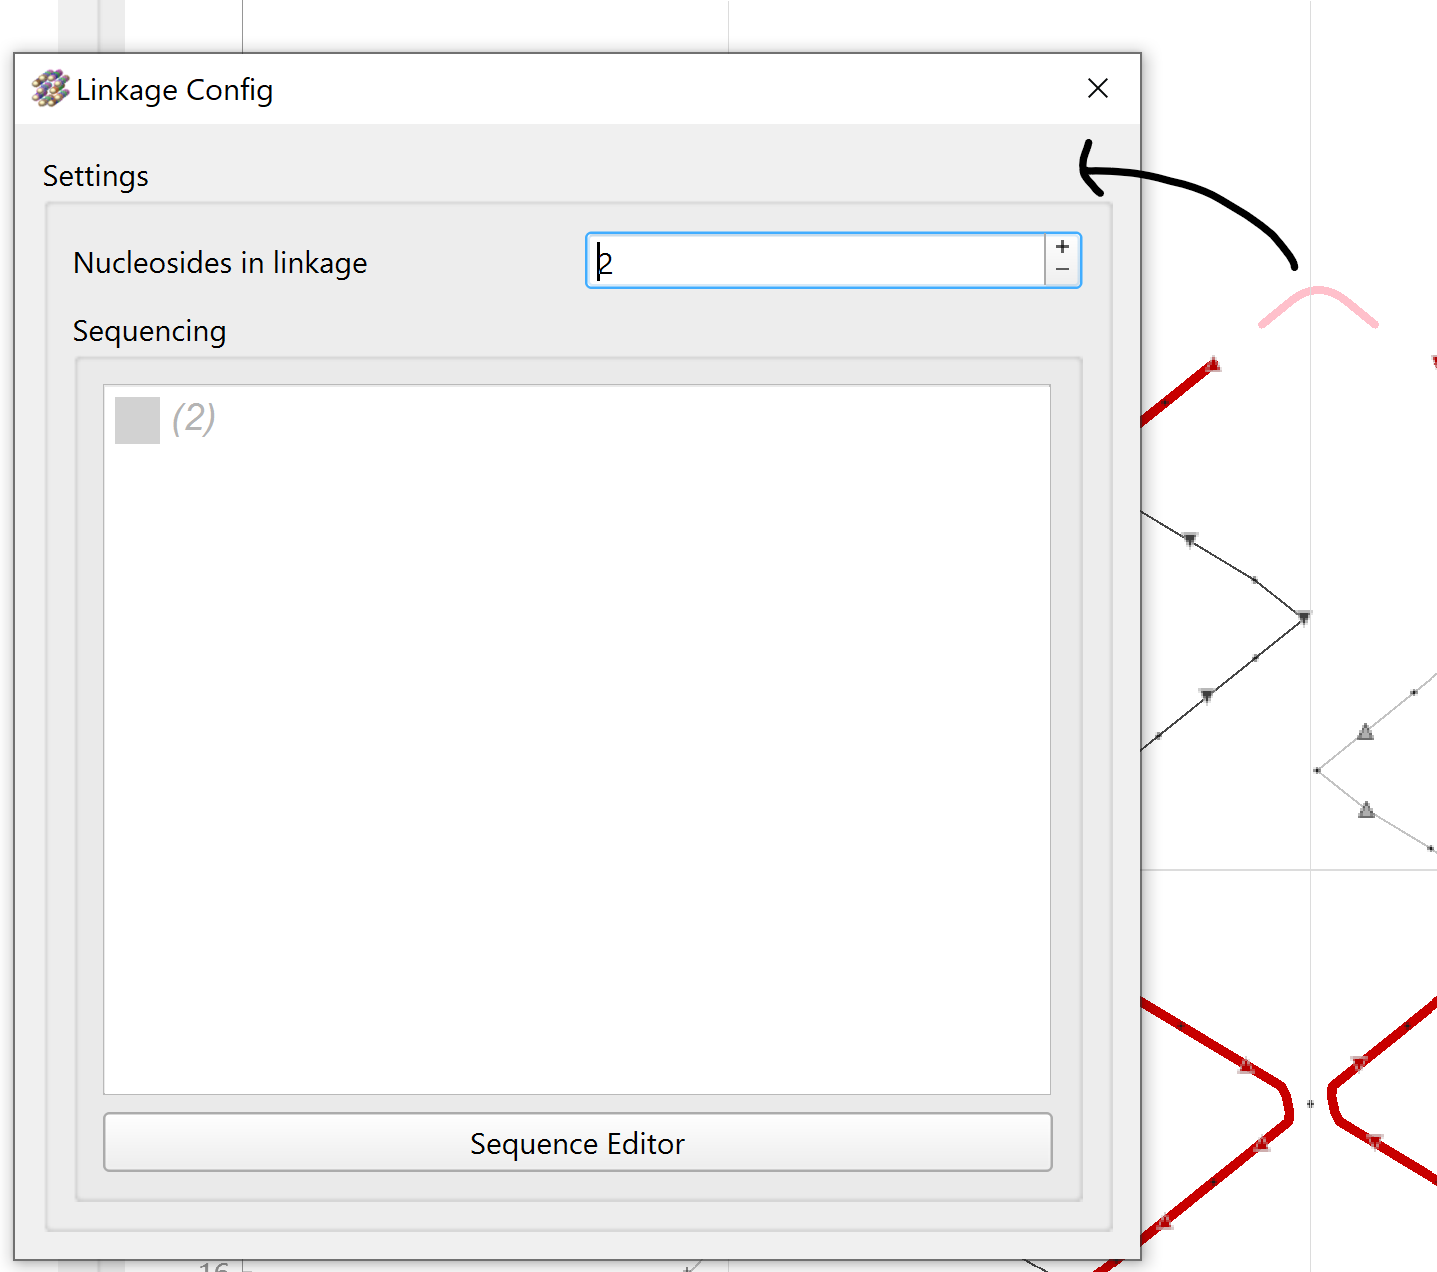
\includegraphics[width=2.3in]{linkage-editor.png}
		\label{fig:linkage-editor}
	\end{figure}

	The "Linker" mode allows you to connect the end of one strand to the beginning of another strand, and vice versa. 
	
	\paragraph{Linkages}
	A linkage is a single-stranded region that connects two formerly distinct strands. In this single-stranded region nucleosides can be added, and bases for those nucleosides can be set. To customize a linkage click on the linkage, and the linkage editor should pop up. The Linkage Editor (see figure~\ref{fig:linkage-editor}) is a dialog that allows you to add nucleosides to the linkage, and to set the sequence of the items in the linkage. To increase or decrease the number of items within the linkage, simply increase the "Nucleosides in Linkage" spinbox, and click tab or enter. Note that the nucleosides in the linkage will show up in the regular strand config sequence editor, but this window only shows the sequence of the items within the linkage.
	
	\begin{figure}[h]
		\centering
		\caption{Linkage creation process}
		\label{fig:linkage-creation-process}
		
		\begin{subfigure}{.3\linewidth}
			\centering
			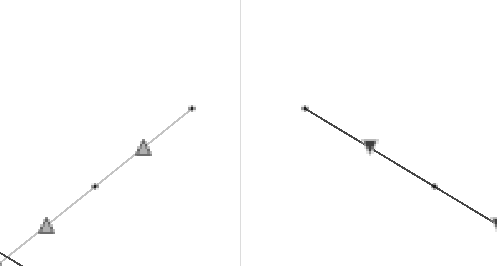
\includegraphics[height=.6in]{pre-linkage.png}
			\caption{Two NEMids that can be linked together}
			\label{fig:nick}
		\end{subfigure}%
		~
		\begin{subfigure}{.3\linewidth}
			\centering
			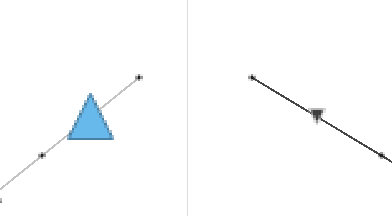
\includegraphics[height=.6in]{pre-linkage-1.png}
			\caption{A selected NEMid that can be linked to another NEMid}
			\label{fig:nick}
		\end{subfigure}%
		~
		\begin{subfigure}{.3\linewidth}
			\centering
			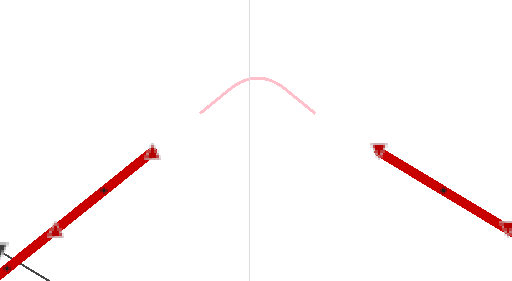
\includegraphics[height=.6in]{linked.png}
			\caption{A completed linkage. This is now one strand.}
			\label{fig:end-of-strand-nick}
		\end{subfigure}
	\end{figure}
	
	To create a linkage:
	\begin{enumerate}
		\item Locate two NEMids that can be made into a linkage. Consult the following list of prerequisites for determining if two NEMids can be linked together---if the following conditions are not met a warning will be displayed.
		\begin{enumerate}
			\item Both NEMids must be endpoints of their respective strands. This means the second to last or second item in their strands (with the nucleoside that follows them being the very last or very first item).
			\item One NEMid is at the 5' end of its strand and the other NEMid is at the 3' end of its strand.
			\item Both strands consist of $>$1 NEMids.
		\end{enumerate}
		\item Left click on one of the NEMids that you would like to link with the other NEMid. The order in which you click the NEMids does not matter. After clicking on a NEMid in linker mode, the NEMid should turn blue and grow larger. This indicates that it is selected.
		\item Left click on the other NEMid that you would like to link it to. A linkage should be created upon releasing left click.
	\end{enumerate}

	\begin{wrapfigure}{r}{.3\linewidth}
		\centering
		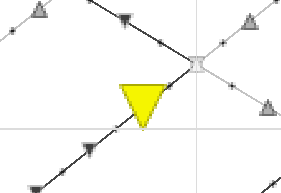
\includegraphics[width=1in]{highlighted-nemid.png}
		\caption{"A highlighted NEMid}
		\label{fig:highlighted-NEMid}
	\end{wrapfigure}

	\subsubsection{Highlighter Mode}

	The "Highlighter" mode lets you highlight points. It makes them larger and yellow, which can be useful for presentations (see figure~\ref{fig:highlighted-NEMid}). 
	To highlight a NEMid or nucleoside, simply click on it. To unhiglight a NEMid or nucleoside, click on the highlighted NEMid or nucleoside a second time.
	
	Notes about highlighting:
	\begin{itemize}
		\item Items will stay highlighted even when you leave highlighter mode. This means that there are actually multiple ways to unhighlight items, including, but not limited to the following.
		\begin{itemize}
			\item Click the highlighted point while in highlighter mode
			\item Create a nick to split the strand in two, or create junction
			\item Click the "Update Graphs" button to refresh the plots
		\end{itemize}
		\item At this time NATuG's highlighting is uncustomizable, so all higlighted items will be large and yellow versions of their past selves.
	\end{itemize}
	
	\section{Top View Plot}
	
	The Top View Plot presents an overhead view of the nanostructure that is currently being created. It allows you to visualize the actual tube shape, and see the interior angles of all the domains. The Top View Plot is a panel, which means that it can be undocked, among other things. For information on panels, see~\ref{sect:panels}.
	
	\begin{figure}[h]
		\centering
		\label{fig:top-view-plot-panel}
		\caption{Top View Plot Panel}
		\begin{subfigure}{.45\linewidth}
			\centering
			\label{fig:top-view-plot-panel-1}
			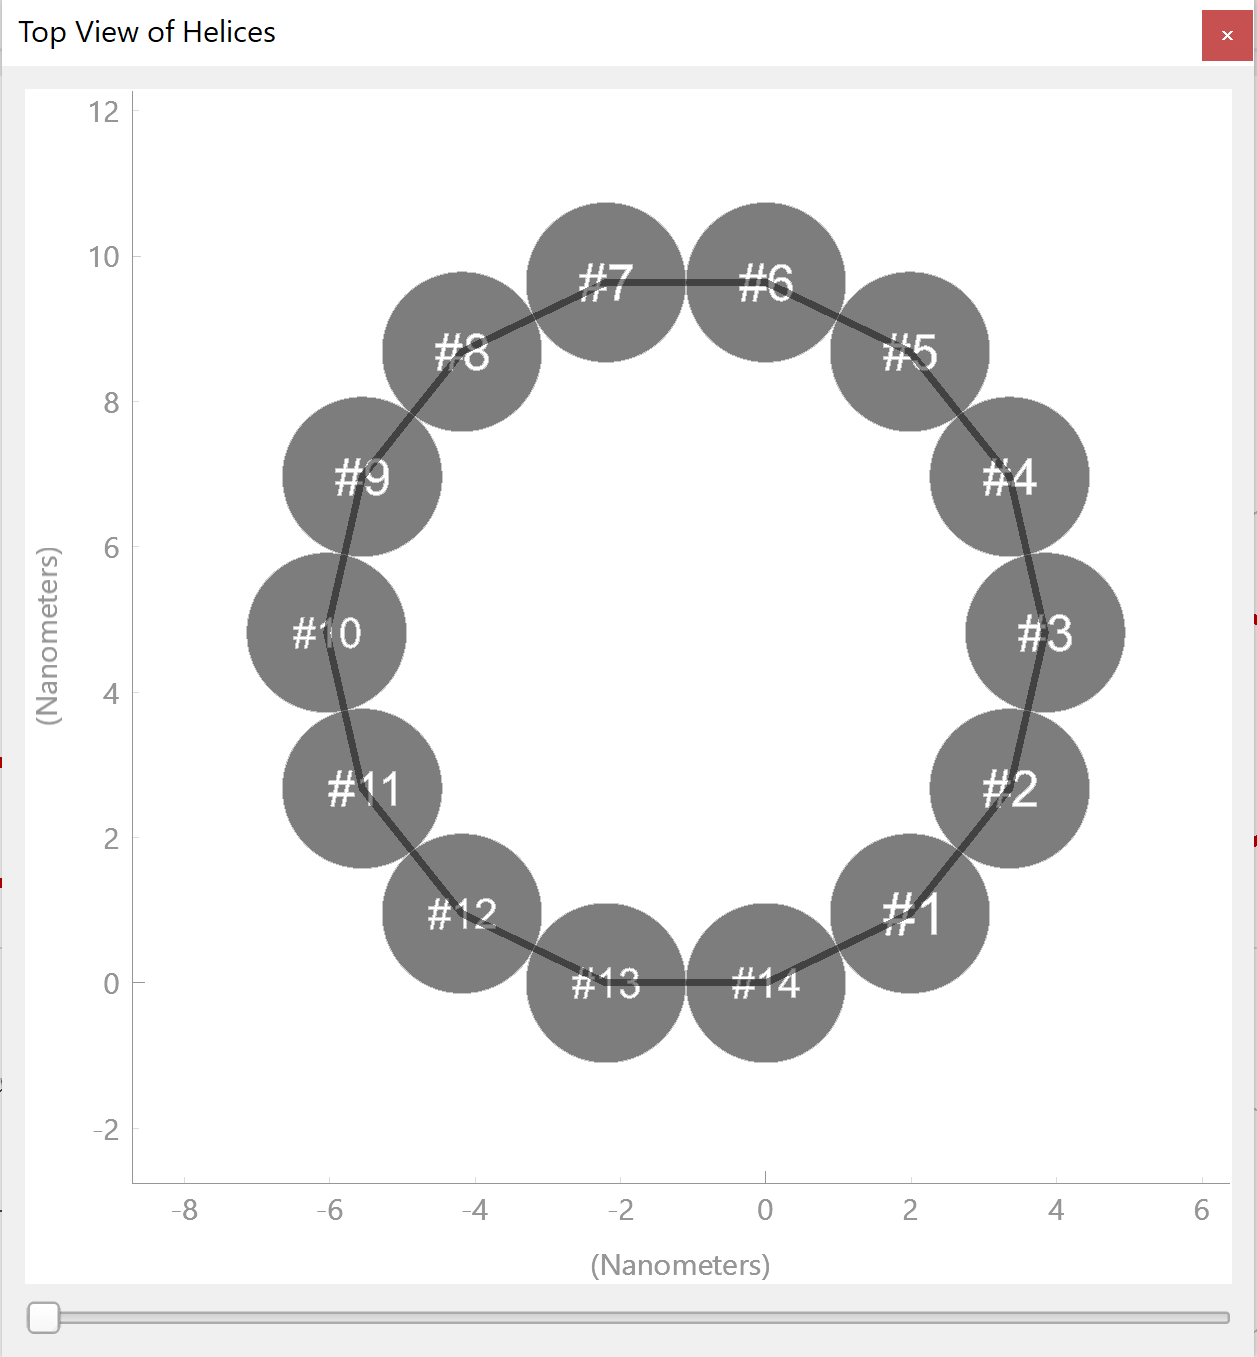
\includegraphics[width=1.8in]{top-view-plot.png}
			\caption{Top View Plot Example 1}
		\end{subfigure}%
		~
		\begin{subfigure}{.45\linewidth}
			\centering
			\label{fig:top-view-plot-panel-2}
			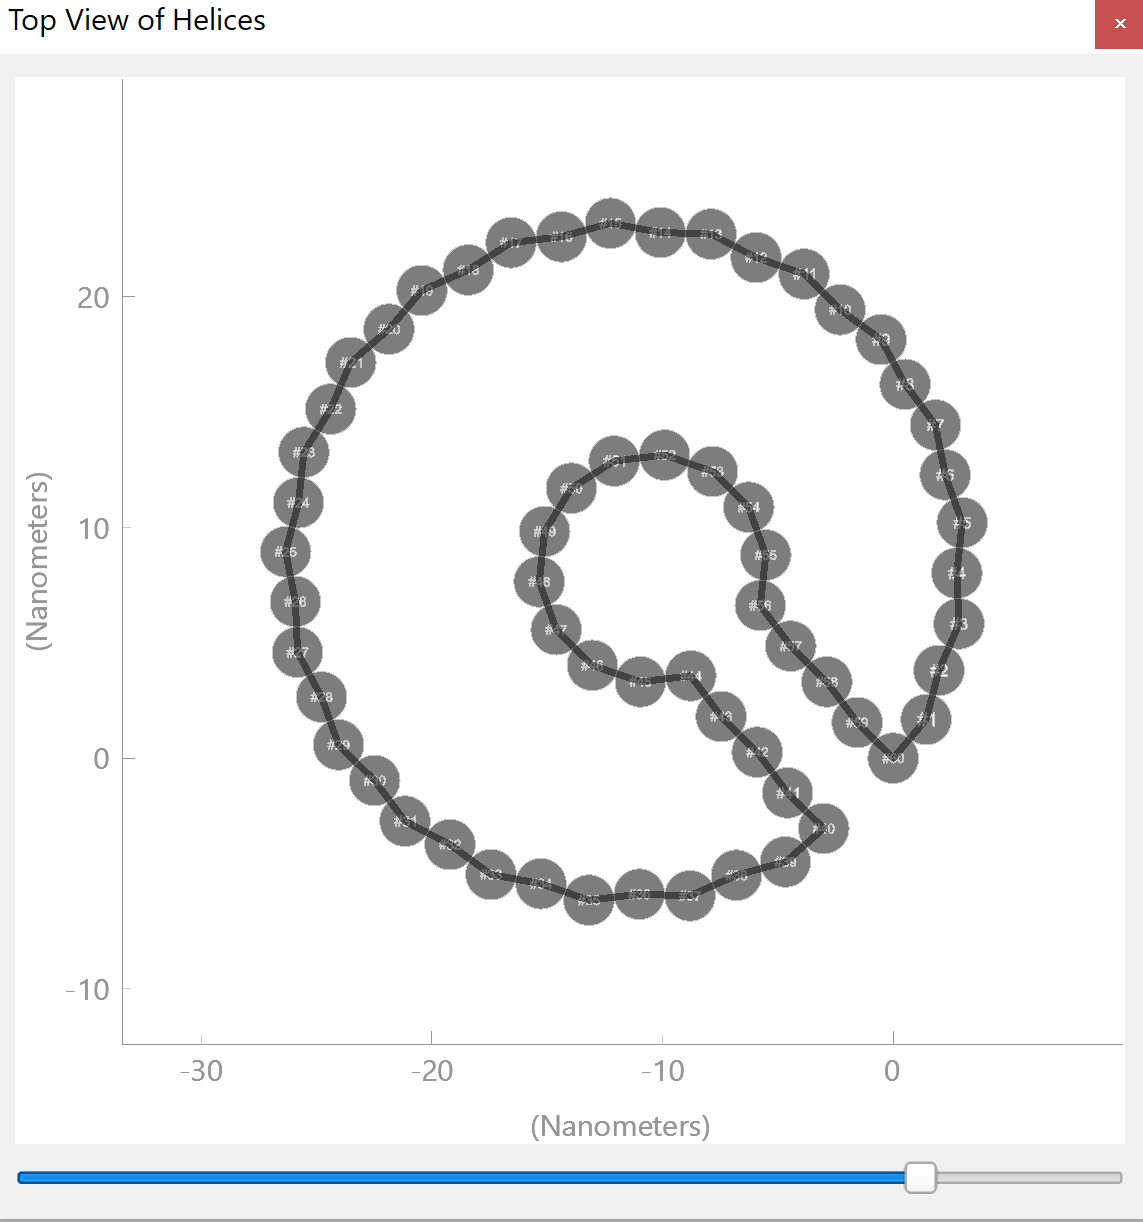
\includegraphics[width=1.8in]{top-view-plot-2.png}
			\caption{Top View Plot Example 2}
		\end{subfigure}
	\end{figure}
	
	\subsection{Graphics}
	In the Top View Plot, each circle represents a helical domain, which is the region in which the double helices exist. The circles are numbered, and the numbers represent the domains' respective indexes. The units of the axes are in nanometers, and depend on the diameter of domains, which can be set in the Nucleic Acid Tab (\ref{sect:nucleic-acid-tab}). An imaginary $0^{th}$ domain is drawn as well to show the last domain's interior angle, but this domain does not actually exist. Additionally, to make it easier to see the interior angles of the domains, a thin line is drawn atop all of the domains' circles.
	
	\subsection{Interaction}
	For the most part, interacting with the Top View Plot is the same as interacting with the Side View Plot (documentation for interaction with the side view plot can be found at~\ref{sect:plot-interaction}). However, there are a few important differences:
	\begin{itemize}
		\item The aspect ratio of the Top View Plot is locked at 1:1. This means that you cannot stretch the plot.
		\item The Top View Plot is rotatable. To rotate the top view plot, drag the handlebar beneath the plot to the right. The left edge of the bar represents a $0^{\circ}$ rotation, and the right edge of the bar represents a $360^{\circ}$ rotation. The plot is rotated after coordinates for all of the domains are computed, and the pivot point of rotation is the middle point of all the domains.
		\item Clicking on a number (not a circle, but rather on a number) will navigate the Side View Plot to the specific domain that was clicked on. Clicking on the same number a second time will restore the full view of the plot.
	\end{itemize}

	\section{Strands}
	
	Whereas a "helix" is specifically a strand that stays within one domain, a "strand" can traverse many domains. When a strand crosses through many domains, it weaves the nanotube together. But, equally important to choosing where the strand goes is determining the base sequence. And, being able to choose styles to represent strands in publications is also critical. This section covers how to customize the properties of a strand.
	
	\subsection{Selecting a Strand}
	
	\begin{figure}[h]
		\centering
		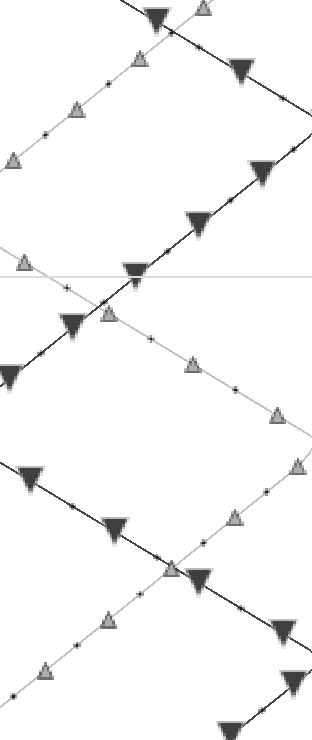
\includegraphics[height=1.4in]{selected-strand.png}
		\label{fig:selected-strand}
		\caption{A selected strand}
	\end{figure}
	
	To select a strand, left click on the line between two NEMids/nucleosides within the Side View Plot. The Strand Config Dialog should pop up, and the NEMids/nucleosides of the strand should grow larger (this is because the width/color of the strand is customizable, so it would be annoying if the strand's color/width changed when highlighting). Only one strand can be selected at a time. Multiple strands can be selected at a time, and the name of the window indicates the strand that the Strand Config Dialog is fore.
	
	\subsection{Configuration}
	
	\begin{figure}[h]
		\centering
		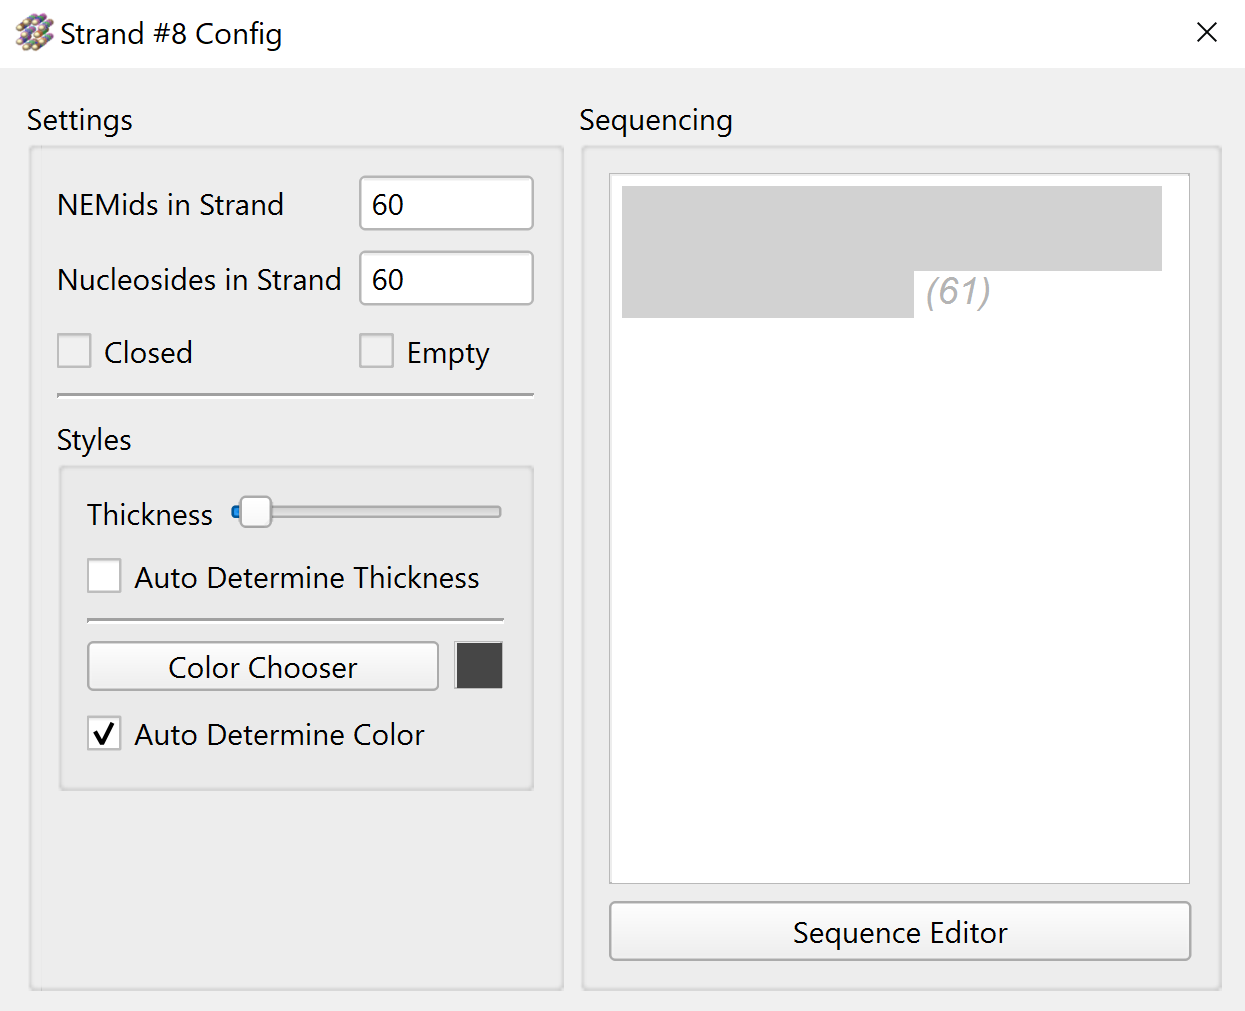
\includegraphics[width=3in]{strand-config.png}
		\caption{Strand Config Dialog}
		\label{fig:strand-config-dialog}
	\end{figure}

	The Strand Config Dialog is the place where you can configure strand styles, obtain additional information about a given strand, and set a strand's sequence. Below there is a detailed description of the three main parts of the strand config dialog:
	
	\paragraph{Settings}
	The settings area of the Strand Config Dialog encompasses the entire left side of the dialog. Within this area, information about the strand can be found, and various styles can be customized.
	
	\subparagraph{Information}
	The information area of the Strand Config Dialog provides the following information about the strand:
	\begin{itemize}
		\item \textbf{NEMids in Strand:} The number of NEMids that are in the strand.
		\item \textbf{Nucleosides in Strand:} The number of nucleosides that are in the strand.
		\item \textbf{Closed:} Whether the strand is a closed loop strand.
		\item \textbf{Empty:} Whether the strand has no items in it. In general, this will be false.
	\end{itemize} 
	In addition, the strand's index in regards to all the other strands (its "id") can be found as the title of the window (see the top of figure~\ref{fig:strand-line})
	
	\subparagraph{Styling}
	The style area of the Strand Config Dialog lets you customize styles of the strand. The styles update in real time, with the exception of the "Automatic" style checkboxes. The "Auto" checkboxes next to the different strand styles tell NATuG whether or not to overright the user-set strand style when refreshing/recoloring the plot. If you want to reset a style of a strand back to the default, select the "Auto" checkbox for the style, and then in the file menu choose "View," and "Restyle Strands."
	
	Below lies a list of the various styles that can be customized, and the default settings of the given styles.
	\begin{itemize}
		\item \textbf{Thickness:} The width of the strand. This is a handlebar that represents the width of the strand in pixels. The very left of the bar represents 1 pixel of thickness, and the very right of the bar represents 50 pixels of thickness. By default, strands that stay in their own domain are 2 pixels thick, and strands that traverse multiple domains are 9.5 pixels thick.
		\item \textbf{Color:} The color of the strand. The "Color Chooser" button creates a Color Chooser Dialog that allows you to select the color of your choosing. Within the dialog, you can enter parameters for your color in RGB/CMYK, choose a screen color, or choose from a preset. By default, strands that stay in their own domain are either light or dark gray, and strands that traverse multiple domains are automatically assigned colors as to keep them distinct from other strands that traverse multiple domains.
	\end{itemize}
	
	\subsection{Sequence Selector} \label{sect:sequence-selector}
		The purpose of the Sequence Selector is to provide a user-friendly way to obtain a valid sequence for a given strand/portion of a strand. Generally, this will pop up when you click a button along the lines of "Choose a Sequence." To use the Sequence Selector, you can either choose to use the Bulk Sequence Input tab, or, if the length of the sequence you are being prompted to choose is under 1,000 bases, the Manual Input Tab. Once you have made your selection of sequence, click the "Load Sequence" button, or click the "Cancel" button to exit the Sequence Selector and cancel the sequence choosing operation. Below, more information about the two areas of the Sequence Selector can be found.
	
	\begin{figure}
		\centering
		\caption{Sequence Selector Dialog}
		\begin{subfigure}{.5\textwidth}
			\centering
			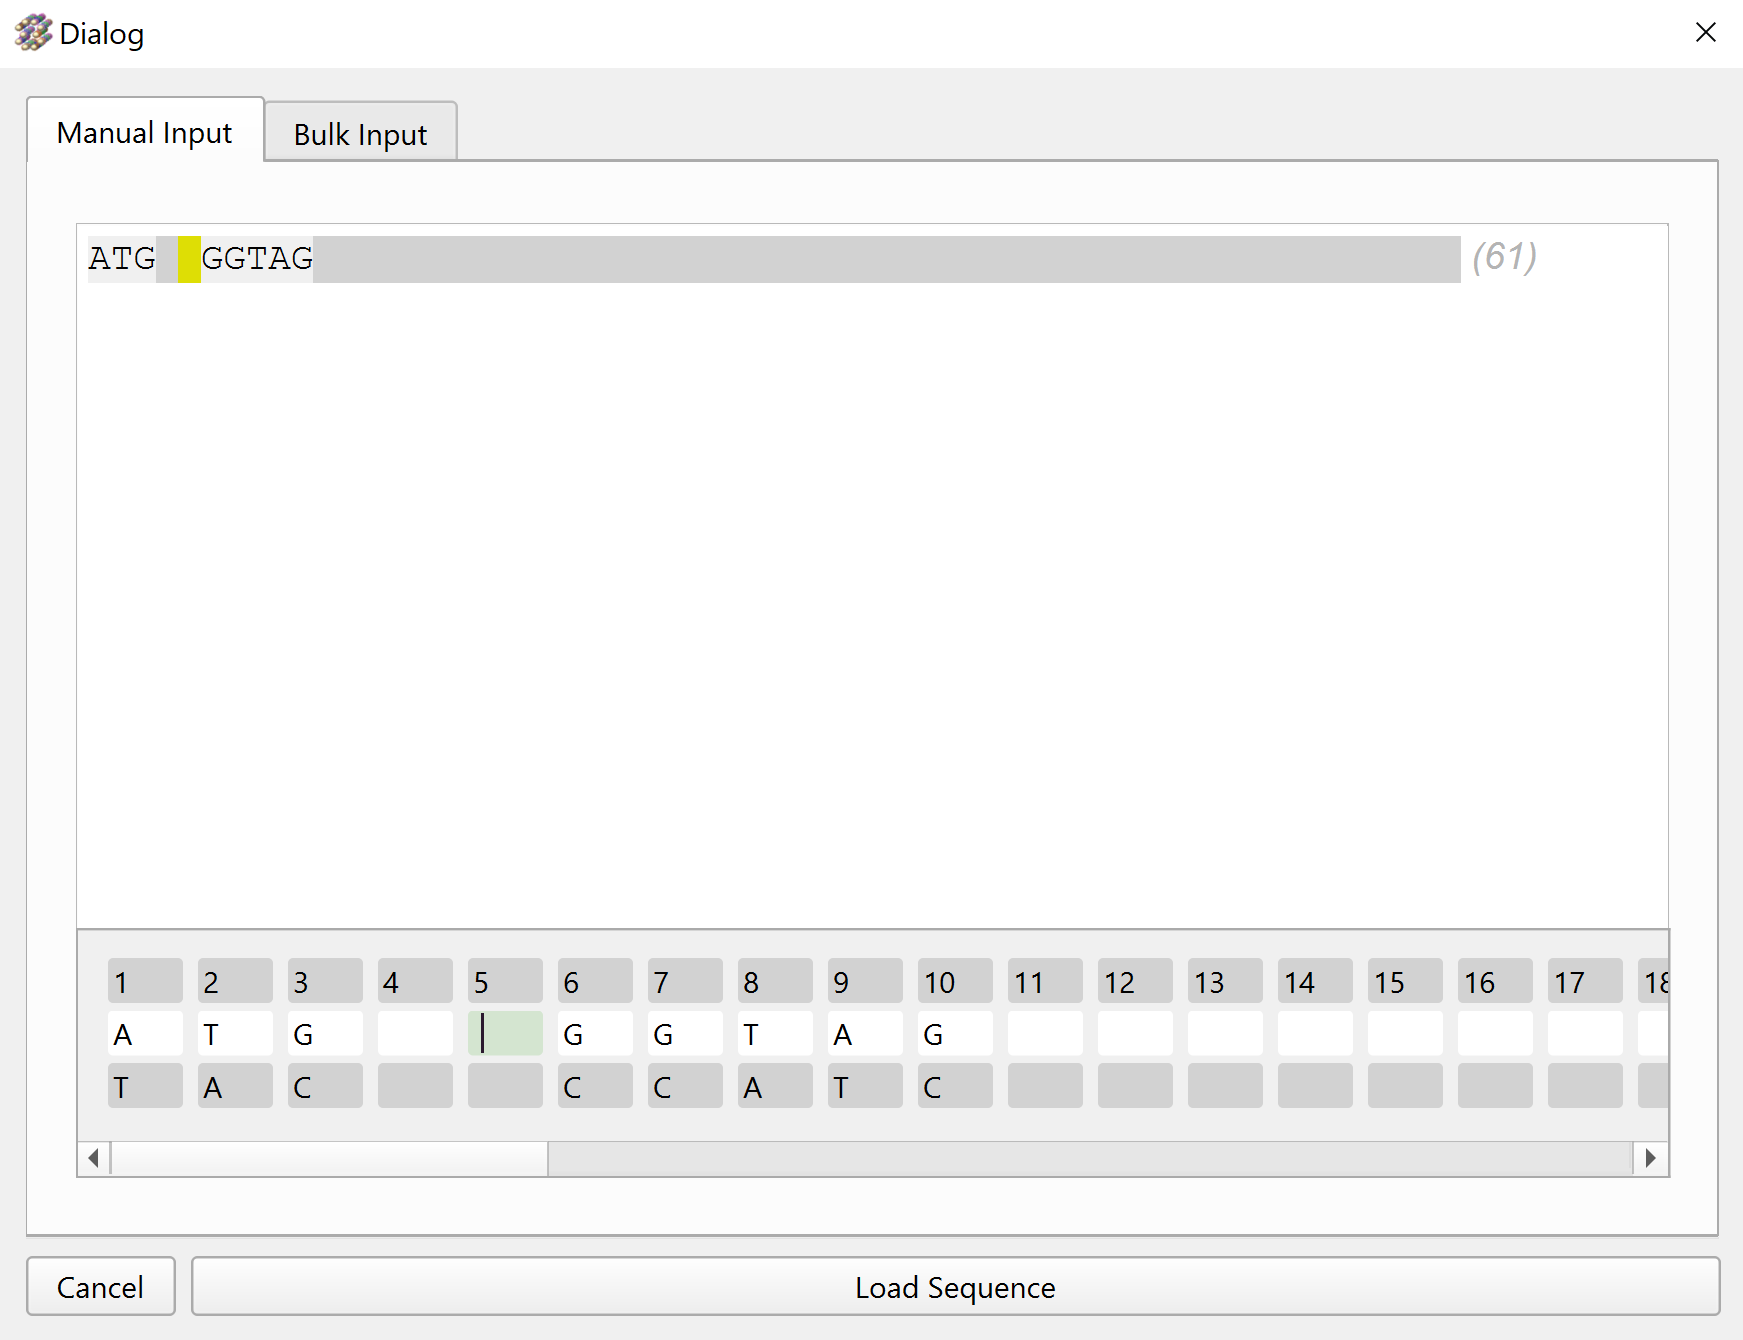
\includegraphics[height=1.8in]{sequence-editor-manual-input.png}
			\caption{Manual Input Tab}
			\label{fig:sequence-dialog-manual-input}
		\end{subfigure}%
		~
		\begin{subfigure}{.5\textwidth}
			\centering
			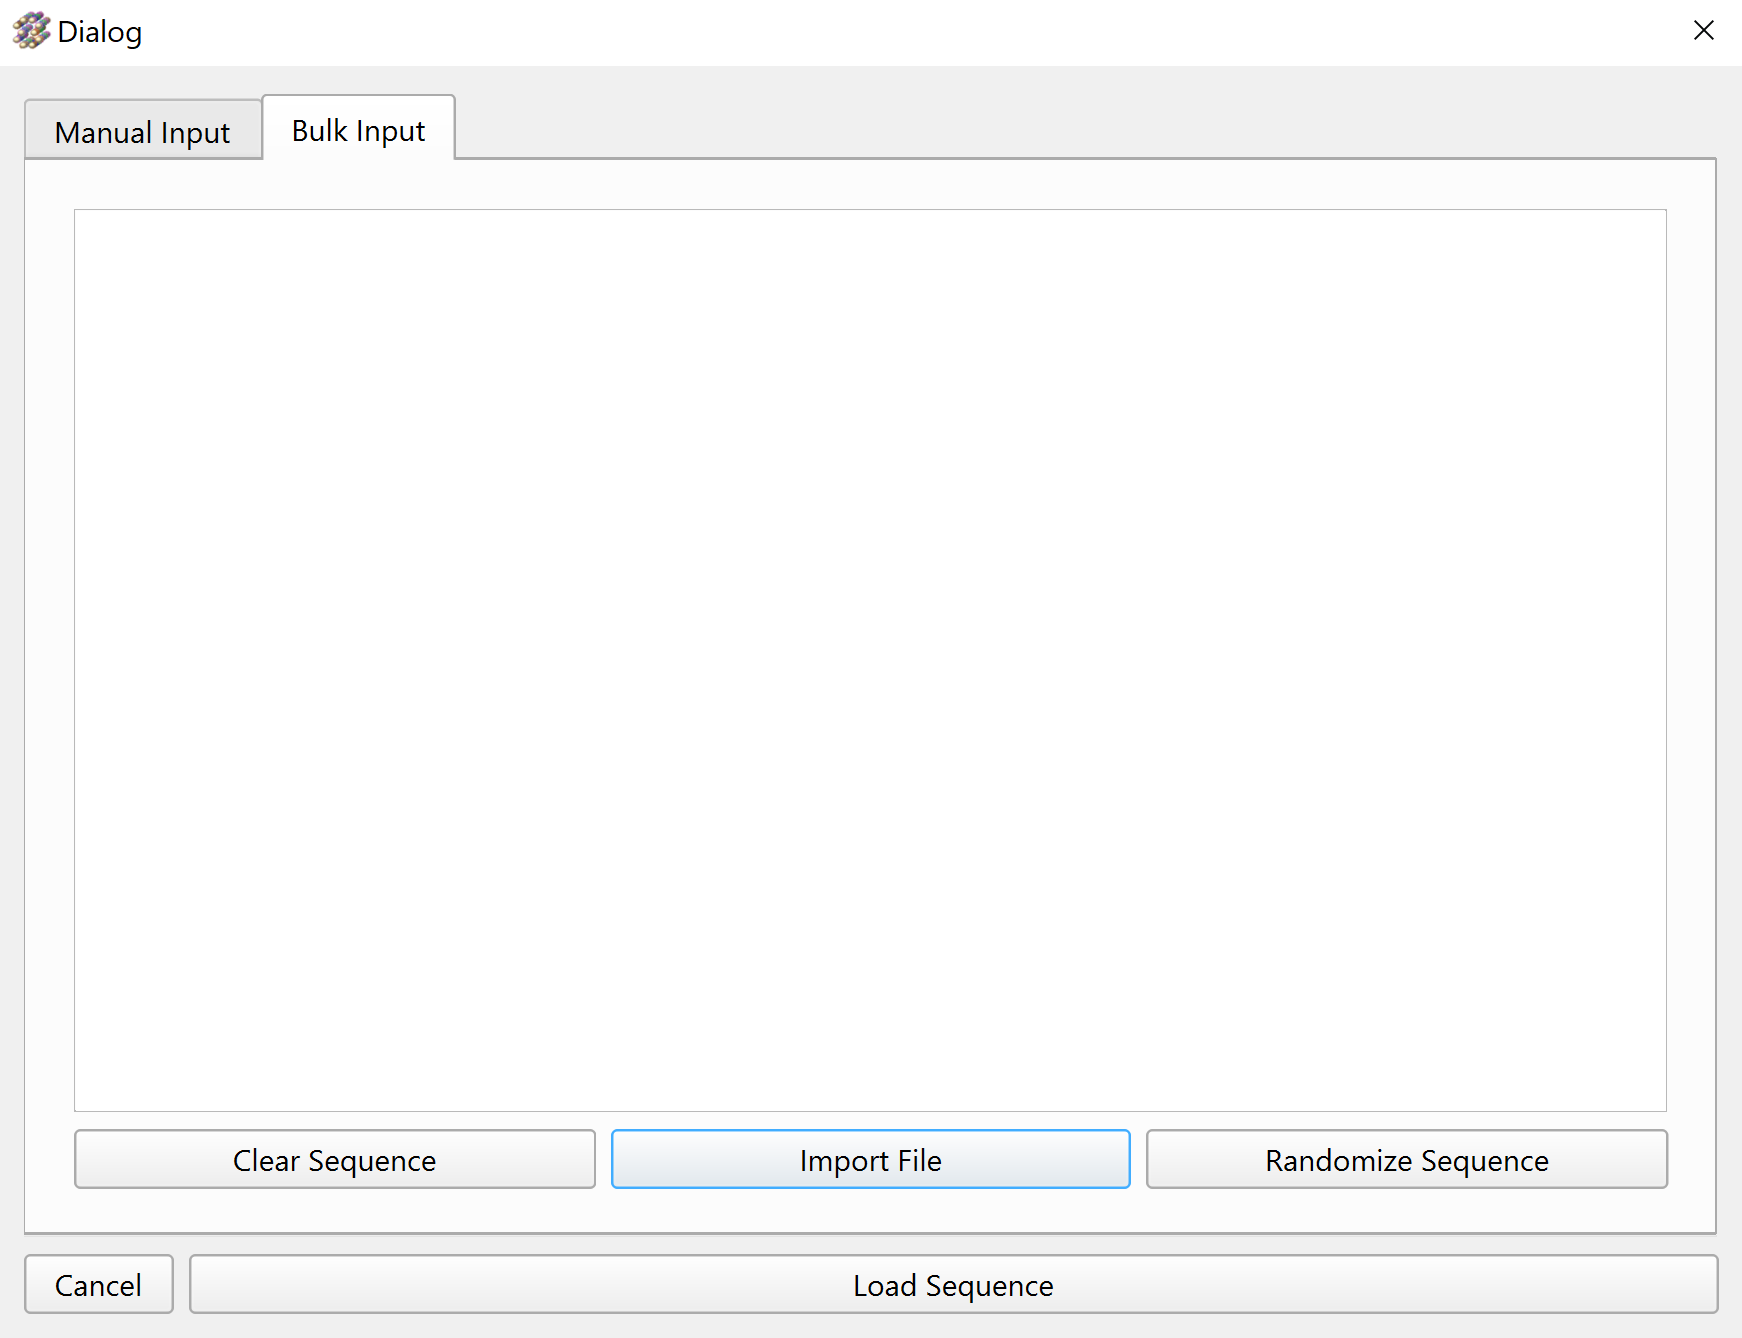
\includegraphics[height=1.8in]{sequence-editor-bulk-input.png}
			\caption{Bulk Input Tab}
			\label{fig:sequence-dialog-bulk-input}
		\end{subfigure}
	\end{figure}

	\subsubsection{Manual Input Tab}
	The Manual Input Tab of the Sequence Selector is like a text editor for a DNA sequence, and makes entering a sequence manually super-simple and convenient. Because of how the Manual Input Tab is implemented, it becomes particularly slow after displaying more than 1,000 bases, so, when more than 1,000 bases need to be set you must use the Bulk Input Tab. The Manual Input tab consists of two main areas, the bottom Sequence Entry Area and the top Sequence Display Area.
	
	\paragraph{Sequence Entry Area}
	The Sequence Entry Area is a horizontally scrollable area that showcases all of the bases currently chosen as editable text boxes. Each white rounded box, also called an Entry Box, represents a single nitrogenous base. The box above each Entry Box is the index of that base. The box below each Entry Box is the complementary base. NATuG uses Watson-Crick base pairing, so the complement of A is T, the complement of T is A, the complement of G is C, the complement of C is G, and the complement of None is None.
	
	When you are using the Sequence Entry Area, you can type into one box at a time either the letter "A," "G," "C," or "T," or you can click the delete key. What you type will automatically be capitalized, and after you enter the letter of a base you will automatically be shifted to the next Entry Box to the right, or, if you enter a base into the last box, you will be shifted to the first Entry Box. As you enter bases into the various Entry Boxes, the Sequence Entry Area will automatically scroll to keep the currently selected box in view.
		
	\paragraph{Sequence Display Area}
	The Sequence Display Area is a larger area that displays the entire current sequence. This area is read only, and highlights the currently selected Entry Box of the Sequence Entry Area. You can select and copy the text of this box, but you cannot edit this box.
	
\end{document}